% Options for packages loaded elsewhere
\PassOptionsToPackage{unicode}{hyperref}
\PassOptionsToPackage{hyphens}{url}
\PassOptionsToPackage{dvipsnames,svgnames,x11names}{xcolor}
%
\documentclass[
  12pt,
]{report}

\usepackage{amsmath,amssymb}
\usepackage{setspace}
\usepackage{iftex}
\ifPDFTeX
  \usepackage[T1]{fontenc}
  \usepackage[utf8]{inputenc}
  \usepackage{textcomp} % provide euro and other symbols
\else % if luatex or xetex
  \usepackage{unicode-math}
  \defaultfontfeatures{Scale=MatchLowercase}
  \defaultfontfeatures[\rmfamily]{Ligatures=TeX,Scale=1}
\fi
\usepackage{lmodern}
\ifPDFTeX\else  
    % xetex/luatex font selection
  \setmainfont[]{Times New Roman}
  \setsansfont[]{Arial}
  \setmonofont[]{Courier New}
\fi
% Use upquote if available, for straight quotes in verbatim environments
\IfFileExists{upquote.sty}{\usepackage{upquote}}{}
\IfFileExists{microtype.sty}{% use microtype if available
  \usepackage[]{microtype}
  \UseMicrotypeSet[protrusion]{basicmath} % disable protrusion for tt fonts
}{}
\usepackage{xcolor}
\usepackage[top=30mm,left=1in,right=1in,bottom=25mm,top = 3cm,bottom =
3cm,left = 3cm,right = 2.7cm]{geometry}
\setlength{\emergencystretch}{3em} % prevent overfull lines
\setcounter{secnumdepth}{5}
% Make \paragraph and \subparagraph free-standing
\ifx\paragraph\undefined\else
  \let\oldparagraph\paragraph
  \renewcommand{\paragraph}[1]{\oldparagraph{#1}\mbox{}}
\fi
\ifx\subparagraph\undefined\else
  \let\oldsubparagraph\subparagraph
  \renewcommand{\subparagraph}[1]{\oldsubparagraph{#1}\mbox{}}
\fi


\providecommand{\tightlist}{%
  \setlength{\itemsep}{0pt}\setlength{\parskip}{0pt}}\usepackage{longtable,booktabs,array}
\usepackage{calc} % for calculating minipage widths
% Correct order of tables after \paragraph or \subparagraph
\usepackage{etoolbox}
\makeatletter
\patchcmd\longtable{\par}{\if@noskipsec\mbox{}\fi\par}{}{}
\makeatother
% Allow footnotes in longtable head/foot
\IfFileExists{footnotehyper.sty}{\usepackage{footnotehyper}}{\usepackage{footnote}}
\makesavenoteenv{longtable}
\usepackage{graphicx}
\makeatletter
\def\maxwidth{\ifdim\Gin@nat@width>\linewidth\linewidth\else\Gin@nat@width\fi}
\def\maxheight{\ifdim\Gin@nat@height>\textheight\textheight\else\Gin@nat@height\fi}
\makeatother
% Scale images if necessary, so that they will not overflow the page
% margins by default, and it is still possible to overwrite the defaults
% using explicit options in \includegraphics[width, height, ...]{}
\setkeys{Gin}{width=\maxwidth,height=\maxheight,keepaspectratio}
% Set default figure placement to htbp
\makeatletter
\def\fps@figure{htbp}
\makeatother
% definitions for citeproc citations
\NewDocumentCommand\citeproctext{}{}
\NewDocumentCommand\citeproc{mm}{%
  \begingroup\def\citeproctext{#2}\cite{#1}\endgroup}
\makeatletter
 % allow citations to break across lines
 \let\@cite@ofmt\@firstofone
 % avoid brackets around text for \cite:
 \def\@biblabel#1{}
 \def\@cite#1#2{{#1\if@tempswa , #2\fi}}
\makeatother
\newlength{\cslhangindent}
\setlength{\cslhangindent}{1.5em}
\newlength{\csllabelwidth}
\setlength{\csllabelwidth}{3em}
\newenvironment{CSLReferences}[2] % #1 hanging-indent, #2 entry-spacing
 {\begin{list}{}{%
  \setlength{\itemindent}{0pt}
  \setlength{\leftmargin}{0pt}
  \setlength{\parsep}{0pt}
  % turn on hanging indent if param 1 is 1
  \ifodd #1
   \setlength{\leftmargin}{\cslhangindent}
   \setlength{\itemindent}{-1\cslhangindent}
  \fi
  % set entry spacing
  \setlength{\itemsep}{#2\baselineskip}}}
 {\end{list}}
\usepackage{calc}
\newcommand{\CSLBlock}[1]{\hfill\break\parbox[t]{\linewidth}{\strut\ignorespaces#1\strut}}
\newcommand{\CSLLeftMargin}[1]{\parbox[t]{\csllabelwidth}{\strut#1\strut}}
\newcommand{\CSLRightInline}[1]{\parbox[t]{\linewidth - \csllabelwidth}{\strut#1\strut}}
\newcommand{\CSLIndent}[1]{\hspace{\cslhangindent}#1}

\usepackage{booktabs}
\usepackage{caption}
\usepackage{longtable}
\usepackage{colortbl}
\usepackage{array}
\usepackage{anyfontsize}
\usepackage{multirow}
\usepackage{sectsty}
\chapterfont{\centering}
\usepackage{lscape}
\newcommand{\blandscape}{\begin{landscape}}
\newcommand{\elandscape}{\end{landscape}}
\makeatletter
\@ifpackageloaded{caption}{}{\usepackage{caption}}
\AtBeginDocument{%
\ifdefined\contentsname
  \renewcommand*\contentsname{Table of contents}
\else
  \newcommand\contentsname{Table of contents}
\fi
\ifdefined\listfigurename
  \renewcommand*\listfigurename{Figures}
\else
  \newcommand\listfigurename{Figures}
\fi
\ifdefined\listtablename
  \renewcommand*\listtablename{Tables}
\else
  \newcommand\listtablename{Tables}
\fi
\ifdefined\figurename
  \renewcommand*\figurename{Figure}
\else
  \newcommand\figurename{Figure}
\fi
\ifdefined\tablename
  \renewcommand*\tablename{Table}
\else
  \newcommand\tablename{Table}
\fi
}
\@ifpackageloaded{float}{}{\usepackage{float}}
\floatstyle{ruled}
\@ifundefined{c@chapter}{\newfloat{codelisting}{h}{lop}}{\newfloat{codelisting}{h}{lop}[chapter]}
\floatname{codelisting}{Listing}
\newcommand*\listoflistings{\listof{codelisting}{List of Listings}}
\makeatother
\makeatletter
\makeatother
\makeatletter
\@ifpackageloaded{caption}{}{\usepackage{caption}}
\@ifpackageloaded{subcaption}{}{\usepackage{subcaption}}
\makeatother
\ifLuaTeX
  \usepackage{selnolig}  % disable illegal ligatures
\fi
\usepackage{bookmark}

\IfFileExists{xurl.sty}{\usepackage{xurl}}{} % add URL line breaks if available
\urlstyle{same} % disable monospaced font for URLs
\hypersetup{
  pdftitle={Leadership Transitions and Survival: Coups, Autocoups, and Power Dynamics},
  pdfauthor={Zhu Qi},
  colorlinks=true,
  linkcolor={blue},
  filecolor={Maroon},
  citecolor={Blue},
  urlcolor={blue},
  pdfcreator={LaTeX via pandoc}}

\title{Leadership Transitions and Survival: Coups, Autocoups, and Power
Dynamics}
\author{Zhu Qi}
\date{}

\begin{document}


\def\spacingset#1{\renewcommand{\baselinestretch}%
{#1}\small\normalsize} \spacingset{1}


%%%%%%%%%%%%%%%%%%%%%%%%%%%%%%%%%%%%%%%%%%%%%%%%%%%%%%%%%%%%%%%%%%%%%%%%%%%%%%

\title{\bf Leadership Transitions and Survival: Coups, Autocoups, and
Power Dynamics}
\author{
Zhu Qi\\University of
Essex\\\href{mailto:qz21485@essex.ac.uk}{qz21485@essex.ac.uk}
}

\maketitle

\bigskip
\bigskip
\begin{abstract}

\end{abstract}


\newpage
\spacingset{1.9} % DON'T change the spacing!
\renewcommand*\contentsname{Contents}
{
\hypersetup{linkcolor=}
\setcounter{tocdepth}{2}
\tableofcontents
}
\listoffigures
\listoftables
\setstretch{1.618}
\chapter*{Acknowledgements}\label{acknowledgements}
\addcontentsline{toc}{chapter}{Acknowledgements}

The completion of this thesis has been a significant journey, filled
with hard work, learning, and moments of joy. Throughout this time, I
have received support and encouragement from many individuals, without
whom this dissertation would not have been possible.

First and foremost, I would like to express my deepest gratitude to my
great supervisor, Professor Kristian Skrede Gleditsch, for his
invaluable guidance, unwavering support, and insightful feedback
throughout this journey. His expertise and encouragement have been
instrumental in shaping this dissertation. I would also like to extend
my heartfelt thanks to the chair of my board panel, Professor Han
Dorussen, for his continuous support and constructive criticism, which
have significantly enhanced the quality of my research.

I am profoundly grateful for the comments, advice, and suggestions from
several esteemed scholars who have contributed to this work. Dr.~Brian J
Phillips, Dr. Prabin Khadka, and Dr.~Winnie Xia, their expertise and
thoughtful input have been greatly appreciated and have enriched this
dissertation.

Finally, I want to thank my family for their unwavering support and
love. To my beloved wife, Ji Zhi, who has been my rock throughout this
journey, and to my dear daughter, Siyan, and son, Sisheng, who have been
my source of joy and motivation. I am deeply thankful to my father for
his enduring support, and to the memory of my late mother, whose love
and guidance continue to inspire me.

All errors and faults are my own.

\chapter*{Abstract}\label{abstract}
\addcontentsline{toc}{chapter}{Abstract}

This dissertation examines the dynamics of irregular power transitions,
particularly coups and autocoups, and their influence on leader
survival. It highlights the critical role of power dynamics, shaped by
\textbf{regime type}, in determining coup success rates and attempt
frequency. Utilizing a \textbf{double probit model with sample
selection}, the study reveals that expected coup success significantly
influences attempts, with military regimes facing a heightened
vulnerability due to their power structure.

While often understudied, autocoups are shown to have a substantial
impact on democratic trends. This research introduces a refined
definition of autocoups alongside a novel dataset encompassing events
from 1945 to 2022, enabling a more robust quantitative analysis.

Employing survival analysis, the study compares the longevity of leaders
who rise to power through coups versus autocoups. The findings
demonstrate that coup-installed leaders face a significantly shorter
tenure and higher risk of removal. This contrasts with autocoup leaders
who manipulate the system to extend their rule, suggesting the potential
for autocoups to incentivize power grabs and contribute to democratic
backsliding.

This work contributes significantly to the political science literature
by:

\begin{itemize}
\item
  Defining key concepts: It establishes a clear definition of autocoups,
  a previously understudied phenomenon.
\item
  Introducing a novel dataset: This dataset enables researchers to
  conduct more comprehensive quantitative analyses of autocoups.
\item
  Establishing a general framework: The framework provides a comparative
  approach to studying the dynamics of irregular power transitions and
  their impact on democratic stability.
\end{itemize}

\textbf{keywords:} \emph{Coups, Autocoups, Power transitions, Leadership
Survival}

\chapter{Introduction}\label{introduction}

\section{Research question}\label{research-question}

Irregular power transitions, marked by a disregard for constitutional
procedures, are a critical area of study in political science. They not
only disrupt established rules but often require unconstitutional
tactics to secure power. Furthermore, these transitions can inspire
copycat behaviour among other ambitious leaders.

Despite their central role in political science and the extensive
research conducted on irregular power transitions, a long-standing
question continues to intrigue political scientists: \textbf{\emph{Why
are some leaders ousted before their terms expire, while others complete
their full terms or even overstay beyond their originally mandated
limits?}} In other words, why do some leaders survive for decades while
others last for only years, months, or even days? This dissertation
focuses on this question and seeks to provide a comprehensive analysis,
dedicated to understanding how leaders come to power through
unconstitutional means and what factors determine the duration of a
leader's rule following an irregular ascent.

\section{Analyses on coups and autocoups in a general
framework}\label{analyses-on-coups-and-autocoups-in-a-general-framework}

When discussing irregular power transitions, the concepts that often
come to mind are irregular entries or exits, such as coups,
assassinations, rebellions, protests, and foreign interventions. Among
these methods, coups hold a prominent position due to their frequent
occurrence. According to the Archigos dataset
(\citeproc{ref-goemans2009}{Goemans, Gleditsch, and Chiozza 2009}), from
1945 to 2015, there were approximately 145 instances of irregular leader
exits, with coups\footnote{According to the Archigos dataset, ``Removed
  by Military, without Foreign Support'' and ``Removed by Other
  Government Actors, without Foreign Support'' in the variable
  \texttt{exitcode} are classified as coups.} accounting for more than
half (79 leaders). The often-cited Global Instances of Coups
(GIC)\footnote{According to the Archigos dataset, ``Removed by Military,
  without Foreign Support'' and ``Removed by Other Government Actors,
  without Foreign Support'' in the variable \texttt{exitcode} are
  classified as coups.} dataset (\citeproc{ref-powell2011}{J. M. Powell
and Thyne 2011}) records even more leaders (245 cases) removed by coups
from 1950 to 2023.

Given their prevalence and substantial influence on political systems,
coups have been extensively studied, particularly since 2000
(\citeproc{ref-thyne2019}{Thyne and Powell 2019}). Consequently, the
concept of a coup is comparatively clear and widely accepted in academic
circles. Many scholars, including this study, follow the definition by
J. M. Powell and Thyne (\citeproc{ref-powell2011}{2011}), which
describes coups as ``illegal and overt attempts by the military or other
elites within the state apparatus to unseat the sitting
executive\ldots{} {[}a coup is successful{]} if the perpetrators seize
and hold power for at least seven days'' (P. 252). Although debates
persist, two elements are clear: first, the perpetrators are elites
within the ruling group, and the victims of coups are incumbent
executive leaders. Second, the strategy or aim of a coup involves
completely removing the incumbents, not merely seizing part of their
power or forcing them to concede on specific policies. Beyond defining
coups, several datasets have been developed for quantitative analyses,
such as the Global Instances of Coups (\citeproc{ref-powell2011}{J. M.
Powell and Thyne 2011}), the Cline Centre Coup d'État Project Dataset
(\citeproc{ref-peyton2024}{Peyton et al. 2024}), and the Colpus Dataset
(\citeproc{ref-chin2021}{Chin, Carter, and Wright 2021}). These datasets
are well-developed and frequently used in political science research.

However, irregular power transitions are not limited to irregular
entries and exits but should also include irregular ``overstays.'' Using
illegal means to overthrow an incumbent leader before their term expires
is undoubtedly an irregular power transition. Similarly, an incumbent
using illegitimate means to extend their term beyond term limits is also
an irregular power transition.

Although academic attention to irregular retention of power has
increased since the 1990s, especially after Peru's President Alberto
Fujimori's self-coup in 1992, it remains comparatively understudied and
has several shortcomings. First, there is no universally accepted
terminology for this ``overstaying in power'' type of irregular power
transition, unlike the clear term ``coup.'' Consequently, various terms
such as self-coup, autogolpe, and executive coup are used by different
scholars. This dissertation will use `autocoup' to refer to this type of
irregular power transition, which will be thoroughly discussed in
Chapter 3. Second, there is no consensus on the definition of an
autocoup. Existing definitions remain vague, often conflating power
expansions and power extensions\footnote{The definitions and concepts of
  power expansion and power extension can be vague. In this study, we
  define power expansion as an incumbent acquiring additional authority
  from other state apparatuses, whereas power extension refers to an
  incumbent prolonging their tenure beyond the designated term in
  office.}. For example, Maxwell A. Cameron
(\citeproc{ref-cameron1998a}{1998a}) defines an autogolpe as a temporary
suspension of the constitution and dissolution of Congress by the
executive, who then rules by decree. This definition focuses on power
expansion instead of power extension, leading to conceptual confusion
and misalignment with the definition of a classic coup. Third, a
consensus autocoup dataset is lacking. While several related datasets
exist, as discussed by Baturo and Tolstrup
(\citeproc{ref-baturo2022}{2022}) in coding their Incumbent Takeover
dataset, the terminologies, definitions, and coverage years vary,
lacking wide acknowledgement and extensive academic exploration. In
summary, autocoup has not been analysed in a comparative manner
connected with coups.

Analysing coups and autocoups separately is less problematic. However,
from a comprehensive framework perspective on irregular power
transitions and leader survival, coups and autocoups should be, and can
be, analysed within the same framework. Both coup and autocoup
significantly influence democratic backsliding and are the most frequent
means of irregular power transition. Furthermore, as both are called
``coups,'' classic coups and autocoups are very similar since a coup is
launched to replace the current leader, while an autocoup is staged to
replace the future leader.

\section{Academic Contributions}\label{academic-contributions}

This study addresses a critical gap in the literature by offering a
comprehensive framework for analysing both coups and autocoups, which
are the most common forms of irregular power transitions. While existing
research often examines these topics separately with varying
terminologies, definitions, methods, and datasets, this dissertation
integrates these elements to provide a unified perspective on irregular
power transitions and leader survival.

Our contributions are threefold:

\begin{itemize}
\item
  \textbf{Emphasis on power dynamics and regime types}: We highlight the
  significant role of power dynamics, particularly the influence of
  regime types, in determining the success and frequency of coup
  attempts. Our analysis underscores how the expected chances of coup
  success motivate such attempts, with military regimes being notably
  susceptible.
\item
  \textbf{Refined definition and novel dataset for autocoups:} We
  introduce a refined definition of autocoups and develop a novel
  dataset covering events from 1945 to 2022. This enables a comparative
  analysis with classic coups, providing clearer insights into the
  nature and impact of autocoups on political systems.
\item
  \textbf{Survival analysis of leaders from different entry modes:} By
  applying survival analysis to existing coup data and our new autocoup
  dataset, we demonstrate how different modes of entry into power
  significantly affect leader survival. Our findings reveal that leaders
  who come to power through coups typically have shorter tenures and
  face higher removal risks compared to those who extend their rule
  through autocoups.
\end{itemize}

Our analysis of irregular power transitions is particularly relevant to
understanding democratic backsliding. These transitions violate
democratic norms and disrupt the path towards stable democracy. Leaders
who gain power through irregular means often employ undemocratic
tactics, such as suppressing opposition, to consolidate their
illegitimate hold on power. This creates a vicious cycle where the
erosion of democratic institutions is both a cause and consequence of
efforts to maintain power.

\section{Overview of the thesis}\label{overview-of-the-thesis}

This study is structured into three main chapters beyond the
introduction, each addressing key aspects of irregular power transitions
and their implications for political stability and democratic processes.

\textbf{Chapter 2} examines the determinants of classic coup attempts.
While extensive research exists on coups, most studies focus on
observable factors before coups, such as economic performance, political
stability, previous coups, and coup-proofing strategies. This chapter,
however, emphasizes the less observable but crucial factor of expected
chances of coup success, which have been often overlooked. Utilizing the
double probit model with sample selection, the analysis reveals that
expected success rates significantly influence coup attempts. These
success rates are primarily shaped by the balance of power between
incumbents and challengers, which is largely determined by regime type.
The findings indicate that military regimes face a much higher risk of
coups compared to dominant-party regimes.

\textbf{Chapter 3} focuses on the concept of autocoups, specifically on
power extensions by incumbent leaders. It distinguishes autocoups from
broader concepts like self-coups or executive coups by redefining them
as instances where incumbent leaders refuse to transition power as
mandated, thereby overstaying in office. Based on this refined
definition, a novel dataset of autocoup events from 1945 to 2022 is
introduced, encompassing 110 attempts and 87 successes. The chapter
includes case studies and empirical analyses that demonstrate the
utility of this dataset for quantitative research, providing a basis for
empirical analysis on autocoups.

\textbf{Chapter 4} investigates how the method of power acquisition
impacts the longevity of leaders who come to power through coups versus
those who extend their rule through autocoups. The hypothesis is that
the method of accession significantly affects leader tenure. Using the
Cox proportional hazards model and a time-dependent Cox model, the
chapter provides evidence of differing survival times between these two
types of leaders. The results indicate that leaders who come to power
through coups face a significantly higher risk of removal compared to
those who extend their rule through autocoups. This finding highlights
the implications for political stability and democratic processes,
suggesting that the relatively low cost and high returns of autocoups
could incentivize incumbents to seize power in this manner, potentially
leading to democratic backsliding and the personalization of power.

In \textbf{Chapter 5}, the study concludes by summarizing the main
findings, discussing policy implications, and acknowledging the
limitations of the research. It also outlines directions for future
research, emphasizing the need for further exploration of irregular
power transitions, particularly coups and autocoups.

\chapter{Power Dynamics and Coup Attempts: A Selection Mechanism
Analysis}\label{power-dynamics-and-coup-attempts-a-selection-mechanism-analysis}

\section{Introduction}\label{introduction-1}

Coups, defined as ``illegal and overt attempts by the military or other
elites within the state apparatus to unseat the sitting executive''
(\citeproc{ref-powell2011}{J. M. Powell and Thyne 2011, 252}), occur
with varying frequency across countries, with some experiencing them
more often than others. According to GIC dataset, Latin American
countries such as Bolivia witnessed 23 coups between 1950 and 1984,
while Argentina experienced 20 during a similar time frame. However,
Mexico's authoritarian period from 1917 to 2000 saw no coups at all. In
Africa, Sudan endured 17 coups between 1955 and 2023, whereas South
Africa has not experienced any coup since 1950. Similar patterns are
observed in the Middle East and South Asia.

The varying frequency of coup attempts has captivated political
scientists for decades, leading to extensive research on the subject. As
highlighted by Gassebner, Gutmann, and Voigt
(\citeproc{ref-gassebner2016}{2016}), despite approximately one hundred
potential determinants of coups being suggested, no consensus has been
reached. In an effort to address this issue, they have tested 66 factors
proposed in previous literature using three million model permutations
in an extreme bounds analysis (ibid.).

Examining previous research, which has tested around 100 variables as
potential determinants of coups, raises an important question beyond
simply understanding why coups are more frequent in some countries than
others. The critical question is: Can we establish a framework to help
scholars focus on the most relevant factors of coups, rather than
sifting through over 100 variables without reaching a consensus?

Reviewing previously proposed variables of coups, it is evident that all
focus on pre-coup conditions, with no consideration given to post-coup
factors. This means more attention is paid to factors observable before
a coup, such as military force or spending, economic performance,
political stability, and previous coups.

\begingroup
\setlength\LTleft{0.05\linewidth}
\setlength\LTright{0.05\linewidth}\fontsize{12.0pt}{14.4pt}\selectfont
\setlength{\LTpost}{0mm}

\begin{longtable}{@{\extracolsep{\fill}}lccr}

\caption{\label{tbl-coups}Top 10 countries with the most coup attempts}

\tabularnewline

\toprule
Country & Coup Attempted & Coup Succeeded & Success Rate \\ 
\midrule\addlinespace[2.5pt]
Bolivia & 23 & 11 & 47.8\% \\ 
Argentina & 20 & 7 & 35.0\% \\ 
Sudan & 17 & 6 & 35.3\% \\ 
Haiti & 13 & 9 & 69.2\% \\ 
Venezuela & 13 & 0 & 0.0\% \\ 
Iraq & 12 & 4 & 33.3\% \\ 
Syria & 12 & 8 & 66.7\% \\ 
Thailand & 12 & 8 & 66.7\% \\ 
Ecuador & 11 & 5 & 45.5\% \\ 
Burundi & 11 & 5 & 45.5\% \\ 
Guatemala & 10 & 5 & 50.0\% \\ 
Total & 491 & 245 & 49.9\% \\ 
\bottomrule

\end{longtable}

\begin{minipage}{\linewidth}
\emph{Source: GIC dataset}\\
\end{minipage}
\endgroup

However, coups are high-stakes gambles with an all-or-nothing nature.
Due to its illegality, the consequences of a failed coup can be severe,
with perpetrators risking imprisonment, exile, or even death. In some
instances, repercussions extend to their families, which means coup
plotters would not take the risk without some assurance of success.

Historical coup attempts and their success rates provide valuable hints
about coup plotters' decision-making processes. Despite the significant
risks associated with coups, as shown in Table~\ref{tbl-coups}, there
have been 491 coups worldwide since 1950. Importantly, about half of
these coups have been successful. At first glance, coups appear to be a
high-success-rate political venture. However, compared to over 12,000
country-years since 1950, the occurrence of 491 coups is relatively
rare, accounting for only about 4\% (GIC).

The low occurrence rate and high success rate clearly indicate that the
initiation of coups is highly selective. In other words, the likelihood
of a coup occurring depends greatly on its probability of success.
However, the probability of success is not a factor that can be observed
before a coup, at least not to outsiders and researchers, but coup
plotters surely have more information on the possible outcome of coups.

Since coup plotters meticulously assess potential outcomes before
staging a coup, coup researchers should also analyse what factors might
affect the outcome of coups. Otherwise, we ran the risk of selection
bias. When considering the factors that most affect the outcomes of
coups, the current literature predominantly identifies military power as
the decisive factor in the success of coups. Ultimately, military power
is determined by the power structure within the regime.

Unlike coup plotters, who have a clearer understanding of power
structures and dynamics, including their supporters, followers,
bystanders, and opponents, researchers are not able to accurately
observe this information. However, we can analyse the most relevant
factors which determine the balance of power and are observable to us.
This leads us to \textbf{regime type}, which reflects the distribution
of power within a government, encompassing who controls the military,
sets policy, and appoints officials. Since coup plotters consider the
balance of power within the regime before acting, this study argues that
regime type plays a crucial role in shaping coup attempts. Analysing
which regime types are more susceptible to coups can offer valuable
insights.

We employ a \textbf{double probit model with sample selection} to
address the selection bias. This model allows us to analyze both the
factors influencing coup success and the factors related to the decision
to initiate a coup attempt in the first place.

This study contributes to the literature in two key ways. First, it
emphasizes the importance of focusing on expected success rates as a
driver of coup attempts, offering a more targeted approach compared to
past studies. Second, it highlights the significance of regime type as a
factor influencing coup likelihood, even when researchers lack perfect
knowledge of a regime's internal power dynamics.

The subsequent section (Section 2) explores the dynamics of coup
attempts and their outcomes. Section 3 delves into the research design,
outlining the methodology and variables used in the analysis. Section 4
presents and discusses the empirical findings. Finally, Section 5
concludes the chapter by summarizing the key insights and their
implications.

\section{Dynamics of coup attempts and
outcomes}\label{dynamics-of-coup-attempts-and-outcomes}

Coup attempts are driven by a complex interplay of factors, including
motivations (\textbf{disposition}) and the resources and opportunities
available to succeed (\textbf{capability}).

\subsection{Motivations for coups}\label{motivations-for-coups}

This section focuses on the motivations that compel challengers to
undertake coups. We can categorize coup motivations into three main
types:

\textbf{Personal Ambition:} Personal ambition is a significant motivator
for the majority of coup plotters, driven by the allure of absolute
power, prestige, and wealth. The prospect of seizing absolute power
provides an unparalleled opportunity to shape national policies, control
resources, and make significant decisions without constraints. The
pursuit of prestige and recognition, along with the potential for
immense economic gain and wealth, further incentivizes individuals.
Additionally, the desire to leave a lasting legacy and make a historical
impact can compel individuals to undertake the risky venture of staging
a coup.

\textbf{Purported National Interest:} Sometimes coups are justified as
necessary interventions to address national crises, uphold the
constitution, or facilitate a transition to democracy. While the
motivations behind such claims require scrutiny, genuine examples do
exist. For instance, the 2010 coup in Niger ousted President Tandja, who
attempted an unconstitutional third term by dissolving the opposing
court and calling a self-serving referendum
(\citeproc{ref-ginsburg2019}{Ginsburg and Elkins 2019}).

\textbf{Self-Preservation:} In some cases, coups serve as pre-emptive
strikes against perceived threats. Coup leaders might not necessarily
seek power, but rather fear elimination or political persecution by the
incumbent regime. An example is Idi Amin's 1971 coup against Ugandan
President Obote, who was attempting to remove Amin from his military
command position (\citeproc{ref-sudduth2017}{Sudduth 2017}).

These motivations are often most prevalent in autocratic regimes, where
justifications under the guise of national interest or self-preservation
can be used to mask personal agendas. Stable democracies rarely face the
same level of constitutional crises or political persecution that might
necessitate a coup. However, new established democracies can be
vulnerable to instability, economic downturns, and democratic
backsliding, creating opportunities for coup plotters to exploit these
weaknesses and justify their actions.

Despite the potential motivations outlined above, coups remain
relatively uncommon, occurring in only about 4\% of country-years since
1950. The main reason is that coup perpetrators face inherent
disadvantages compared to incumbent leaders, highlighting the importance
of capability. Even the most motivated plotters need the resources and
opportunities to succeed. The next section will explore the concept of
capability in greater detail.

\subsection{Capability for coups}\label{capability-for-coups}

For coup plotters, the decision to act hinges not only on their
motivations but also on a calculated assessment of their chances of
success. Several factors can influence this threshold:

\begin{itemize}
\item
  \textbf{Military Strength}: A clear advantage in military capabilities
  compared to the incumbent regime significantly increases the odds of a
  successful coup.
\item
  \textbf{Internal Divisions within the Regime}: Existing fractures
  within the government's power structure can present opportunities for
  coup plotters to exploit weaknesses and gain support from disgruntled
  factions.
\item
  \textbf{Public Support}: Widespread discontent with the incumbent
  regime, especially within the military or key sectors of society, can
  create an environment ripe for a successful coup.
\item
  \textbf{Foreign Backing}: External support from powerful nations can
  provide resources, legitimacy, and even direct military intervention
  to tip the scales in favour of the coup plotters.
\end{itemize}

The high success rate of coups since 1950, as shown in
Table~\ref{tbl-coups}, might suggest that coups are not particularly
difficult to succeed. However, it is important to consider selection
bias. We only observe attempted coups, not the numerous dispositions and
conspiracies that never came to light. Analysing launched coup data
alone can be misleading.

To gain a more comprehensive understanding of coup attempts and their
likelihood, we need to move beyond historical data and employ a
theoretical framework that accounts for selection bias. This framework
will allow us to analyze the factors influencing both the success of
coups and the decision to attempt a coup in the first place. The next
section will delve into such a framework and its implications for our
understanding of coup attempts.

\subsection{Framework of coup success}\label{framework-of-coup-success}

An oft-cited framework (\citeproc{ref-gassebner2016}{Gassebner, Gutmann,
and Voigt 2016}; \citeproc{ref-aidt2019}{Aidt and Leon 2019}) provides a
structured approach to assess the disposition and capability of coup
attempts by evaluating the anticipated benefits for coup plotters. The
expected pay-off of coups can be represented by the equation:

\begin{equation}\phantomsection\label{eq-eq1}{
\begin{aligned}
E(U) = p \times B + (1 - p) \times (-C)
\end{aligned}
}\end{equation}

Here, \(\mathbf B\) represents the return of a successful coup,
\(\mathbf C\) signifies the cost of a failed coup, and \(p\) represents
the probability of coup success. The condition for staging a coup is
when the expected benefit is positive, meaning that the expected pay-off
is greater than 0. Rearranging the equation, we get:

\begin{equation}\phantomsection\label{eq-eq2}{
\begin{aligned}
p \times B > (1 - p) \times C
\end{aligned}
}\end{equation}

Equation~\ref{eq-eq2} implies that for Equation~\ref{eq-eq1} to hold,
the expected benefits earned from successful coups must outweigh the
expected cost of failed coups.

While seemingly clear, the equation faces practical challenges.
Quantifying \(\mathbf B\) (the value of a successful coup) and
\(\mathbf C\) (the cost of failure) is difficult. The loss of life,
freedom, or loved ones after a failed coup, as well as the value of
assuming leadership after a successful coup, are intangible concepts
that defy precise measurement. As evidenced by the 1979 coup in
Ghana\footnote{According to the Archigos dataset, ``Removed by Military,
  without Foreign Support'' and ``Removed by Other Government Actors,
  without Foreign Support'' in the variable \texttt{exitcode} are
  classified as coups.}, the fate of the coup leader(s) hangs in the
balance; they are high likely to be killed if the coup fails, or to
execute others if the coup succeeds.

However, these challenges do not render the framework useless. Firstly,
its core logic remains valuable, offering insights into how coup
plotters might assess the return and cost of their actions. Secondly,
given the significant and elusive nature of precise values for
\(\mathbf B\) and \(\mathbf C\), they can be treated as roughly equal.
Consequently, there is no need to fret over how to measure and compare
these values precisely. Instead, we can shift our focus from
\(\mathbf B\) and \(\mathbf C\), to the probability of success (\(p\)),
simplifying Equation~\ref{eq-eq2} to:

\begin{equation}\phantomsection\label{eq-eq3}{
\begin{aligned}
p > (1-p)
\end{aligned}
}\end{equation}

Equation~\ref{eq-eq3} suggests that, to hold Equation~\ref{eq-eq2} true,
a success probability greater than \(50\%\) is necessary. Interestingly,
empirical data on coups since 1950 somewhat supports this notion. As
shown in Table~\ref{tbl-coups}, the overall success rate is \(49.9\%\).
While this falls short of the \(50\%\) threshold, it's important to
consider two factors. Firstly, this is an average rate, not necessarily
reflective of the probabilities assessed by coup plotters beforehand.
Secondly, outliers such as irrational actors and coups driven by
self-preservation may not prioritize success probabilities. Taking these
points into account, we can propose our first hypothesis:

\begin{quote}
\textbf{\emph{H1: The fundamental determinant of a coup attempt is the
perceived chance of success. Coup plotters likely require a success
threshold of at least 50\%.}}
\end{quote}

This leads us to the next crucial question: What factors determine coup
success, influencing the very decision to attempt one? We will discuss
it in the next section.

\subsection{Regime types and power
dynamics}\label{regime-types-and-power-dynamics}

The high success rate in historical data is merely a post-event
statistical description, not indicative of the probability of any
specific coup. Importantly, coup plotters do not rely on past success
rates as their guide; instead, they assess their chances based on their
unique context.

Military strength undeniably plays a critical role in coup attempts.
Control of the armed forces offers a significant advantage, explaining
why military coups dominate discussions on the topic. Much of the
literature treats ``coup'' and ``military coup'' interchangeably, with
scholars like J. M. Powell and Thyne (\citeproc{ref-powell2011}{2011})
finding that half of 14 studies attribute coups solely to the military.
Consequently, significant focus, from both researchers and
policy-makers, centres on the balance of power between civilian and
military authorities, or among military factions themselves. Strategies
like ``keeping the military content'' (\citeproc{ref-aidt2019}{Aidt and
Leon 2019}) or ``providing them with resources''
(\citeproc{ref-huntington1991democratization}{Huntington 1991}) aim to
reduce military intervention. Empirical research informs coup-proofing
strategies that either decrease the military's desire for coups or raise
barriers to success (\citeproc{ref-leon2013a}{Leon 2013};
\citeproc{ref-powell2018}{J. Powell et al. 2018}).

However, while military power is decisive, it complicates the analysis.
As Table~\ref{tbl-regimes} demonstrates, military regimes, despite
concentrated military control, exhibit surprising instability,
experiencing the most frequent coup attempts. This highlights a crucial
issue: the intra-military component. Treating the military as a
monolithic entity ignores its complex internal dynamics
(\citeproc{ref-singh2016}{Singh 2016}). Any military comprises diverse
groups with their own hierarchies, fostering suspicion, competition, and
vigilance rather than unity. The clandestine nature of coups
necessitates small, secretive groups. Plotters are unsure of other
factions' stances and fear their opposition or intervention, as
exemplified by the swiftly thwarted 2021 Niger coup\footnote{The
  definitions and concepts of power expansion and power extension can be
  vague. In this study, we define power expansion as an incumbent
  acquiring additional authority from other state apparatuses, whereas
  power extension refers to an incumbent prolonging their tenure beyond
  the designated term in office.}. The success of a coup hinges heavily
on other military factions' reactions (\citeproc{ref-geddes1999}{Geddes
1999}).

Moreover, military force is not the only factor shaping the balance of
power. Internal divisions within the ruling elites, public support, and
foreign backing also play important roles. Since the balance of power is
not a clearly observable variable, especially difficult to measure for
outsiders and academic scholars, we can shift our focus from who
controls power in a specific context to what factors shape the balance
of power. This leads us to regime type, as the classification of regime
type is based mainly on the power structure. For example,
``\ldots definition of regimes emphasizes the rules that identify the
group from which leaders can come and determine who influences
leadership choice and policy'' (\citeproc{ref-geddes2014}{Geddes,
Wright, and Frantz 2014, 314}). We will leverage this framework to
categorize autocracies based on leadership origin and decision-making,
classifying regimes into three main categories: military, personalist,
and dominant-party.

\begin{itemize}
\item
  \textbf{Military Regimes:} Characterized by the dominance of a
  junta---a group of military officers who control the regime's power
  structure, including leadership selection and policy formulation.
  Examples include the Brazilian regime (1964-1985), the Argentine
  regime (1976-1983), and the Salvadoran regime (1948-1984)
  (\citeproc{ref-geddes1999}{Geddes 1999}).
\item
  \textbf{Personalist Regimes:} Power resides with a single, charismatic
  leader who controls policy, the military, and succession. Regimes like
  Rafael Trujillo's in the Dominican Republic (1930-1961), Idi Amin's in
  Uganda (1971-1979), and Jean-Bédel Bokassa's in the Central African
  Republic (1966-1979) exemplify personalist rule (ibid.).
\item
  \textbf{Dominant-Party Regimes:} Power rests within a well-organized
  ruling party, with leaders acting as its representatives. The party
  structure and ideology foster internal cohesion and a long-term
  vision. Examples include the Partido Revolucionario Institucional
  (PRI) in Mexico, the Revolutionary Party of Tanzania (CCM), and
  Leninist parties in various Eastern European countries (ibid.).
\end{itemize}

The critical distinction between regime types lies in the unique power
balance established during their seizure of power, often through
irregular and violent means, frequently involving military
confrontations. This power struggle typically results in the emergence
of the most competent group---be it a military junta, a political party,
or a strongman---as the core leadership. Furthermore, the early stages
of new regimes are often marked by internal purges to consolidate power
and eliminate potential rivals (\citeproc{ref-sudduth2017}{Sudduth
2017}; \citeproc{ref-roessler2011}{Roessler 2011}).

Following these external challenges and internal purges, new power
dynamics emerge in three primary forms: dominant-party regimes,
personalist regimes, and military regimes. These contrasting power
dynamics significantly influence a regime's susceptibility to coups.
Dominant-party regimes, characterized by a well-organized party with
clear ideology, hierarchy, and discipline, exhibit the greatest
resilience against coups due to their institutionalized structures and
unified leadership. Personalist regimes, where power centers around a
single strong leader, are relatively stable during the leader's tenure.
However, they face a higher risk of coups, particularly due to the lack
of clear succession plans and vulnerabilities associated with the
leader's personal weaknesses, health issues, and finite lifespan.
Military regimes, characterized by power struggles within a junta, are
the most vulnerable to coups. The absence of a clear final authority in
military regimes often leads to internal conflicts, and the presence of
multiple military factions increases the likelihood of resolving
disputes through force, making these regimes the least stable.
Table~\ref{tbl-regimes1} summarises the key characteristics of the three
main regime types.

These contrasting power dynamics significantly influence a regime's
susceptibility to coups. As Table~\ref{tbl-regimes} confirms, military
regimes, despite representing only 5.6\% of country-years, experience a
disproportionate share of coups, accounting for over 22\% of all
occurrences. Personalist regimes face a similarly high coup risk,
constituting 23\% of coups while representing only 13\% of
country-years. Conversely, dominant-party regimes, with their
institutionalized structures and unified leadership, exhibit the
greatest resilience. They represent 22.6\% of country-years but account
for only 16.7\% of coups. The column ``Coup Likelihood'' clearly
illustrates the varying risks: military regimes have the highest
likelihood at 17.2\%, followed by personalist regimes at 7.7\%, and
dominant-party regimes at 3.2\% (excluding \emph{Other} regime types).

\begin{quote}
\textbf{\emph{H2: Due to their balance of power dynamics, military
regimes are more prone to coups, followed by personalist regimes, while
dominant-party regimes are the least likely to experience coups among
the three.}}
\end{quote}

\newpage

\blandscape

\begingroup
\setlength\LTleft{0\linewidth}
\setlength\LTright{0\linewidth}\fontsize{12.0pt}{14.4pt}\selectfont
\setlength{\LTpost}{0mm}

\begin{longtable}{@{\extracolsep{\fill}}>{\raggedright\arraybackslash}p{\dimexpr 75.00pt -2\tabcolsep-1.5\arrayrulewidth}>{\raggedright\arraybackslash}p{\dimexpr 75.00pt -2\tabcolsep-1.5\arrayrulewidth}>{\raggedright\arraybackslash}p{\dimexpr 75.00pt -2\tabcolsep-1.5\arrayrulewidth}>{\raggedright\arraybackslash}p{\dimexpr 75.00pt -2\tabcolsep-1.5\arrayrulewidth}>{\raggedright\arraybackslash}p{\dimexpr 75.00pt -2\tabcolsep-1.5\arrayrulewidth}>{\raggedright\arraybackslash}p{\dimexpr 75.00pt -2\tabcolsep-1.5\arrayrulewidth}}

\caption{\label{tbl-regimes1}Main features of different types of
regimes}

\tabularnewline

\toprule
Regime Type & Power Concentration & Succession & Military Alignment & Stability & Examples \\ 
\midrule\addlinespace[2.5pt]
Military & Junta & Unclear & May have significant influence & Low & Brazil (1964-1985), Argentina (1976-1983) \\ 
Personalist & Single Leader & Unclear or dependent on leader's will & Subordinated to leader & Moderate (initially), Low (long-term) & Dominican Republic (Trujillo, 1930-1961) \\ 
Dominant-Party & Party Leadership & Institutionalized & Aligned with the party & High & Mexico (PRI), China (CPC) \\ 
\bottomrule

\end{longtable}

\begin{minipage}{\linewidth}
\emph{Source: GWF \& Author}\\
\end{minipage}
\endgroup

\newpage

\begingroup
\setlength\LTleft{0\linewidth}
\setlength\LTright{0\linewidth}\fontsize{12.0pt}{14.4pt}\selectfont
\setlength{\LTpost}{0mm}

\begin{longtable}{@{\extracolsep{\fill}}lrrrrrr}

\caption{\label{tbl-regimes}Regime types and coups since 1950}

\tabularnewline

\toprule
Regime Type & Country Year & Share & Num of Coups & Percent of Coups & Success Rate & Coup Likelihood \\ 
\midrule\addlinespace[2.5pt]
Democracy & 5303 & 46.7\% & 122 & 24.8\% & 51.6\% & 2.3\% \\ 
Dominant-Party & 2569 & 22.6\% & 82 & 16.7\% & 53.7\% & 3.2\% \\ 
Personal & 1477 & 13.0\% & 113 & 23.0\% & 44.2\% & 7.7\% \\ 
Monarchy & 1056 & 9.3\% & 25 & 5.1\% & 56.0\% & 2.4\% \\ 
Military & 638 & 5.6\% & 110 & 22.4\% & 48.2\% & 17.2\% \\ 
Other & 322 & 2.8\% & 39 & 7.9\% & 53.8\% & 12.1\% \\ 
Total & 11365 & 100.0\% & 491 & 100.0\% & 49.9\% & 4.3\% \\ 
\bottomrule

\end{longtable}

\begin{minipage}{\linewidth}
\emph{Source: REIGN and GIC Datasets}\\
\end{minipage}
\endgroup

\elandscape

\section{Research Design}\label{research-design}

\subsection{Double probit with sample selection
model}\label{double-probit-with-sample-selection-model}

This study employs a sophisticated statistical approach to account for
the selective nature of coup attempts. While coup attempt rates vary
across regimes (as discussed previously), success rates tend to be
surprisingly consistent, hovering around 50\% (as shown in
Table~\ref{tbl-regimes}). This suggests that coup attempts are not
random acts, but rather strategically planned and undertaken only when
the odds of success appear favourable. A standard statistical model
would not account for this selectivity, potentially leading to biased
results.

To address this issue, we utilize a two-stage sample selection model,
similar to the approach used by J. Powell
(\citeproc{ref-powell2012}{2012}). This model has two parts:

\begin{itemize}
\item
  \textbf{Selection Equation (Stage 1):} This stage analyzes the factors
  influencing whether a coup attempt occurs in a particular regime. The
  primary explanatory variable here is regime type, as previously
  discussed. Additional control variables may also be included, denoted
  by \(\mathbf{XB}\).
\item
  \textbf{Outcome Equation (Stage 2):} This stage focuses on the
  probability of success for those coup attempts that actually take
  place.
\end{itemize}

The primary explanatory variables are regime types, as previously
discussed. Control variables are included in \(\mathbf{XB}\). The
selection equation (first stage) models the probability that a coup
attempt occurs and can be expressed as follows:

\begin{equation}\phantomsection\label{eq-eq4}{
\begin{aligned}
y_1^*=\alpha_0 + \alpha_1 Regime_i + \mathbf {XA} + \mu_{1i}
\end{aligned}
}\end{equation}

Here, \({y_1}^*\) is an unobserved variable, which may be known to coup
plotters. \(Regime_i\) is a categorical variable (\emph{military},
\emph{personalist}, or \emph{dominant-party}). \(\mathbf{XB}\) captures
other control variables, such as the economic crisis index, previous
coups, military expenditure, etc.

The observed binary outcome \(\mathbf{y_1}\) is:

\[
\begin{aligned}
y_1 = 
\begin{cases} 
1 &\text{if $y_1^*>0$ (coup attempt occurs)} \\
0 &\text{if $y_1^*\le0$ (no coup attempt)}
\end{cases}
\end{aligned}
\]\\
In the first stage, if \(y_1^*\le0\), no coup attempt occurs in a given
country-year, indicating that the unobserved variable does not reach the
threshold. If \(y_1^*>0\), at least one coup attempt is made in a
country-year, indicating that the unobserved variable surpasses the
threshold. The probability is expressed as:

\begin{equation}\phantomsection\label{eq-eq4a}{
\begin{aligned}
Prob(y_1 =1)&=Prob(y_{1}^*>0) \\
&=\Phi(\alpha_0 + \alpha_1 Regime_i + \mathbf{XA})
\end{aligned}
}\end{equation}

Similarly, the outcome equation (second stage) models the probability
that a coup attempt is successful, given that it occurs:

\begin{equation}\phantomsection\label{eq-eq5}{
\begin{aligned}
y_2^*=\beta_0 + \beta_1 Regime_i + \mathbf {XB} + \mu_{2i}
\end{aligned}
}\end{equation}

The observed outcome \(y_2\) is:

\[
\begin{aligned}
y_2 = 
\begin{cases} 
1 &\text{if $y_2^*>0$ (coup succeeds)} \\
0 &\text{if $y_2^*\le0$ (coup fails)}
\end{cases}
\end{aligned}
\]

The probability equations is:

\begin{equation}\phantomsection\label{eq-eq5a}{
\begin{aligned}
Prob(y_2=1|y_1 =1)=\Phi(\beta_0 + \beta_1 Regime_i + \mathbf{XB})
\end{aligned}
}\end{equation}

\subsection{Variables}\label{variables}

\begin{itemize}
\tightlist
\item
  Dependent variable
\end{itemize}

Our analysis utilizes data on coup attempts and outcomes from J. M.
Powell and Thyne (\citeproc{ref-powell2011}{2011}). A successful coup is
defined as one where the incumbent leader is removed from power for more
than seven days. The dataset covers the period from 1950 to 2023 and
includes information on 491 coup attempts, with roughly half (245) being
successful. Descriptive statistics for these coup attempts and regime
types can be found in Table~\ref{tbl-coups} and Table~\ref{tbl-regimes}.

\begin{itemize}
\tightlist
\item
  Key Independent Variable: Regime Type
\end{itemize}

The core variable of interest is regime type, categorized following the
classification system of Geddes, Wright, and Frantz
(\citeproc{ref-geddes2014}{2014}) (GWF). We focus on military,
personalist, and dominant-party regimes, with democracies and monarchies
included for comparison. Descriptive statistics for regime types are
presented in Table~\ref{tbl-regimes}.

\begin{itemize}
\tightlist
\item
  Control variables
\end{itemize}

Our control variables are chosen based on the research of Gassebner,
Gutmann, and Voigt (\citeproc{ref-gassebner2016}{2016}). They analyzed
66 factors potentially influencing coups and found that slow economic
growth, prior coup attempts, and other forms of political violence are
particularly significant factors. Therefore, we include economic
performance, political violence, and the number of previous coups as our
main control variables.

\textbf{Economic Performance:} We measure economic performance using the
current-trend (\(CT\)) ratio developed by Krishnarajan
(\citeproc{ref-krishnarajan2019}{2019}). This ratio compares a country's
current GDP per capita to the average GDP per capita over the previous
five years. A higher \(CT\) ratio indicates stronger economic
performance. We use GDP per capita data (in constant 2017 international
1000 dollars, PPP) from the V-Dem dataset by Fariss et al.
(\citeproc{ref-fariss2022}{2022}), lagged by one year to reflect the
prior year's economic impact. For a country \(i\) at year \(t\), the
\(CT\) ratio is calculated as follows: \[
\begin{aligned}
CT_{i,t} = {GDP/cap_{i,t} \over {1 \over 5} {\sum_{k=1}^5GDP/cap_{i,t-k}}}
\end{aligned}
\]

\textbf{Political Violence:} We capture overall regime stability by
including a violence index that encompasses all types of internal and
interstate wars and violence. This data comes from the Major Episodes of
Political Violence dataset by Marshall
(\citeproc{ref-marshall2005current}{Marshall 2005}).

\textbf{Previous coups:} The number of previous coups in a country is
included in the first-stage (selection) model to assess its influence on
the likelihood of a coup attempt. However, it is excluded from the
second-stage model (outcome) because the number of past coups may not
directly impact the outcome of a specific coup attempt. Recognizing that
previous coups from a long time ago might not significantly affect the
current situation, I ran another regression using the time distance
since the last coup instead of the number of previous coups for
comparison. This approach accounts for the diminishing impact of past
events over time, providing a potentially more accurate assessment of
how historical coup activity influences the likelihood of current coup
attempts.

\section{Results and Discussion}\label{results-and-discussion}

\begin{table}[!htbp] \centering 
  \caption{Sample Selection Model of Regime Types and Coups, 1950-2019} 
  \label{results} 
\small 
\begin{tabular}{@{\extracolsep{7pt}}lcccc} 
\\[-1.8ex]\hline 
\hline \\[-1.8ex] 
\\[-1.8ex] & \multicolumn{2}{c}{Model 1} & \multicolumn{2}{c}{Model 2} \\ 
 & Coup Attempts & Coup Outcome & Coup Attempts & Coup Outcome \\ 
\\[-1.8ex] & (1) & (2) & (3) & (4)\\ 
\hline \\[-1.8ex] 
 Constant & $-$1.774$^{***}$ & $-$1.803$^{***}$ & $-$1.663$^{***}$ & $-$0.653 \\ 
  & (0.058) & (0.360) & (0.088) & (0.518) \\ 
  & & & & \\ 
 Regime: Democracy & 0.056 & 0.068 & 0.043 & 0.042 \\ 
  & (0.072) & (0.121) & (0.075) & (0.192) \\ 
  & & & & \\ 
 \hspace{1.6cm}Military & 0.687$^{***}$ & 0.596$^{***}$ & 0.345$^{***}$ & 0.247 \\ 
  & (0.084) & (0.170) & (0.091) & (0.229) \\ 
  & & & & \\ 
 \hspace{1.6cm}Monarchy & 0.282$^{**}$ & 0.178 & 0.234$^{*}$ & 0.088 \\ 
  & (0.118) & (0.201) & (0.123) & (0.310) \\ 
  & & & & \\ 
 \hspace{1.6cm}Personalist & 0.319$^{***}$ & 0.128 & 0.134$^{*}$ & $-$0.145 \\ 
  & (0.075) & (0.170) & (0.080) & (0.205) \\ 
  & & & & \\ 
 Economic trend & $-$0.015$^{***}$ & $-$0.004 & $-$0.014$^{***}$ & 0.009 \\ 
  & (0.002) & (0.007) & (0.002) & (0.008) \\ 
  & & & & \\ 
 GDP per capita & $-$0.028$^{***}$ & $-$0.028$^{***}$ & $-$0.016$^{***}$ & $-$0.016 \\ 
  & (0.003) & (0.006) & (0.003) & (0.010) \\ 
  & & & & \\ 
 Political violence & 0.033$^{**}$ & 0.033$^{*}$ & 0.038$^{***}$ & 0.025 \\ 
  & (0.013) & (0.020) & (0.013) & (0.031) \\ 
  & & & & \\ 
 Previous coups (P) & 0.030$^{***}$ &  & 0.447$^{***}$ &  \\ 
  & (0.010) &  & (0.086) &  \\ 
  & & & & \\ 
 Yrs since coup (Y) &  &  & $-$0.018$^{***}$ &  \\ 
  &  &  & (0.004) &  \\ 
  & & & & \\ 
 Interaction term: P * Y &  &  & $-$0.013$^{***}$ &  \\ 
  &  &  & (0.005) &  \\ 
  & & & & \\ 
\hline \\[-1.8ex] 
Observations & 9,606 & 9,606 & 9,606 & 9,606 \\ 
Log Likelihood & $-$1,663.646 & $-$1,663.646 & $-$1,598.603 & $-$1,598.603 \\ 
$\rho$ & 0.898$^{***}$  (0.158) & 0.898$^{***}$  (0.158) & 0.386$^{*}$  (0.234) & 0.386$^{*}$  (0.234) \\ 
\hline 
\hline \\[-1.8ex] 
\textit{Note:}  & \multicolumn{4}{r}{$^{*}$p$<$0.1; $^{**}$p$<$0.05; $^{***}$p$<$0.01} \\ 
\end{tabular} 
\end{table}

The double \texttt{probit} model with sample selection, estimated using
the \texttt{sampleSelection} package
(\citeproc{ref-sampleSelection-2}{Toomet and Henningsen 2008}) in R,
provides valuable insights into the factors influencing coup attempts
and their outcomes across different regime types from 1950 to 2019
(Table \ref{results}). We present two models that differ slightly in
their treatment of previous coups: Model 1 incorporates the number of
previous coups, while Model 2 utilizes the time elapsed since the last
coup.

\newpage

\subsection{The Selection Model: Coup
Attempts}\label{the-selection-model-coup-attempts}

\begingroup
\setlength\LTleft{0.025\linewidth}
\setlength\LTright{0.025\linewidth}\fontsize{12.0pt}{14.4pt}\selectfont
\setlength{\LTpost}{0mm}

\begin{longtable}{@{\extracolsep{\fill}}llrr}

\caption{\label{tbl-mfx1}Average marginal effects of coup attempts
(Selection of Model 1)}

\tabularnewline

\toprule
Term & Contrast & AME\textsuperscript{\textit{1}} & Ratio Percent \\ 
\midrule\addlinespace[2.5pt]
Regime: Democracy & mean(democracy - dominant-party) & 0.003 & 13.030 \\ 
{\hspace{47.25pt}Military} & mean(military - dominant-party) & 0.070 & 277.730 \\ 
{\hspace{47.25pt}Monarchy} & mean(monarchy - dominant-party) & 0.020 & 80.620 \\ 
{\hspace{47.25pt}Personal} & mean(personal - dominant-party) & 0.024 & 93.980 \\ 
Economic trend & mean(+1) & -0.001 & -2.850 \\ 
GDP per capita & mean(+1) & -0.002 & -5.400 \\ 
Political violence & mean(+1) & 0.003 & 6.550 \\ 
Previous coups & mean(+1) & 0.002 & 5.930 \\ 
\bottomrule

\end{longtable}

\begin{minipage}{\linewidth}
\textsuperscript{\textit{1}}AME: Average Marginal Effect\\
\end{minipage}
\endgroup

In the selection model (Column 1), military and personalist regimes
exhibit significant positive coefficients at the 1\% level, indicating a
higher likelihood of experiencing coup attempts compared to
dominant-party regimes. Control variables also exhibit effects in
expected directions. Stronger economic performance, indicated by higher
economic growth trends and GDP per capita levels, correlates with a
lower risk of coup attempts. This suggests that better economic
conditions and relatively higher living standards reduce incentives for
coups. Political violence shows a positive and significant effect on
coup attempts, indicating that higher levels of instability increase the
likelihood of coups. The positive coefficient for the number of previous
coups suggests a ``copycat'' effect from earlier incidents.

While interpreting \texttt{probit} model results directly is not
intuitive, Table~\ref{tbl-mfx1}, generated using
\texttt{marginaleffects} package
(\citeproc{ref-marginaleffects}{Arel-Bundock, Greifer, and Heiss NaN}),
helps clarify the regime effects. The Average Marginal Effect (AME)
column shows changes in probability when a variable increases by one
unit (for numeric variables) or compared to a reference category (for
categorical variables). For instance, the military regime's marginal
effect of 0.07 indicates that the probability of coup attempts in
military regimes is 7 percentage points (pp) higher than in
dominant-party regimes, ceteris paribus. For GDP per capita, the
marginal effect of -0.002 suggests that a \$1000 increase reduces the
probability of coup attempts by 0.2 pp under average conditions.

The Ratio column displays the relative change in percent. While a 7 pp
increase might seem modest, it is substantial in context. Given that the
average probability of a coup attempt in dominant-party regimes is
approximately 2.53\%, the 7 pp increase means military regimes are about
277.7\% more likely to encounter coups than dominant-party regimes---a
significant change. Similarly, personalist regimes show a 2.4 pp higher
probability, about 94\% more likely compared to dominant-party regimes.
Monarchies display a positive effect similar to personalist regimes,
reflecting that monarchies are essentially a subset of personalist
regimes with royal titles.

Control variables, however, show weak effects in predicting coup
attempts. None of their marginal effects reach 1 pp in probability, and
all are less than 7\% in ratio. Given that the actual probability of a
coup attempt is only 2\% to 3\%, these small increases or decreases can
be considered negligible.

These results align with our theoretical expectations regarding internal
power struggles within military juntas and succession vulnerabilities in
personalist regimes, underscoring the importance of regime structure in
understanding coup likelihood.

Model 2 employs years since the last coup instead of the number of
previous coups. Due to most countries not experiencing coups, an
interaction term between previous coups (as a binary variable indicating
presence or absence of coups) and years since the last coup is used.
Generally, Model 2 shows results in the same direction as Model 1,
albeit with relatively lower coefficients (Table~\ref{tbl-mfx2}).

\begingroup
\setlength\LTleft{0.025\linewidth}
\setlength\LTright{0.025\linewidth}\fontsize{12.0pt}{14.4pt}\selectfont
\setlength{\LTpost}{0mm}

\begin{longtable}{@{\extracolsep{\fill}}llrr}

\caption{\label{tbl-mfx2}Average marginal effects of coup attempts
(Selection of Model 2)}

\tabularnewline

\toprule
Term & Contrast & AME\textsuperscript{\textit{1}} & Ratio Percent \\ 
\midrule\addlinespace[2.5pt]
Regime: Democracy & mean(democracy - dominant-party) & 0.003 & 8.930 \\ 
{\hspace{47.25pt}Military} & mean(military - dominant-party) & 0.028 & 91.650 \\ 
{\hspace{47.25pt}Monarchy} & mean(monarchy - dominant-party) & 0.018 & 57.040 \\ 
{\hspace{47.25pt}Personal} & mean(personal - dominant-party) & 0.009 & 30.090 \\ 
Economic trend & mean(+1) & -0.001 & -2.530 \\ 
GDP per capita & mean(+1) & -0.001 & -2.890 \\ 
Political violence & mean(+1) & 0.003 & 7.330 \\ 
Previous coups (P) & mean(1 - 0) & 0.023 & 91.990 \\ 
NA & mean(+1) & -0.002 & -5.050 \\ 
\bottomrule

\end{longtable}

\begin{minipage}{\linewidth}
\textsuperscript{\textit{1}}AME: Average Marginal Effect\\
\end{minipage}
\endgroup

\subsection{The Outcome Model: Coup
Success}\label{the-outcome-model-coup-success}

The outcome model (Columns 2 and 4 in Table \ref{results}) reveals
determinants of coup success. Military regimes demonstrate a higher
probability of coup success compared to dominant-party regimes, aligning
with expectations that military regimes face higher coup risks due to
their increased chances of success. Personalist and monarchical regimes
show slight positive effects on coup success, but these effects are not
statistically significant.

Control variables exhibit different patterns in the outcome model
compared to the selection model. Both GDP per capita and political
violence maintain a weak influence, similar to their effects in the
selection model. However, the economic trend shows a less significant
negative effect on coup success.

These results indicate that regime type remains a significant
determinant of both coup attempts and successes, even after controlling
for other factors, strongly supporting the proposed theoretical
framework.

\subsection{Discussion}\label{discussion}

The \(\rho\) values of 0.898 in Model 1 and 0.386 in Model 2,
significant at 1\% and 10\% levels respectively, are crucial parameters
in the sample selection model. These values represent the correlation
between the error terms of the selection equation (coup attempts) and
the outcome equation (coup outcomes). A high and significant \(\rho\)
suggests that unobserved factors influencing the likelihood of a coup
attempt are strongly correlated with those influencing the likelihood of
a successful coup. Practically, this indicates that the selection model
is appropriate and that accounting for selection bias (i.e., the fact
that only coups with high chances of success will be attempted) is
critical for obtaining unbiased estimates. The high \(\rho\) value
indicates that the same underlying conditions that lead to a coup
attempt also affect its success, underscoring the importance of
considering both stages in the analysis.

The results strongly support the choice of the sample selection model.
Significant coefficients with theoretically consistent directions
suggest the model effectively captures key aspects of coup dynamics.
Regimes with weaker institutional structures are more vulnerable to coup
attempts, while better economic conditions make coups less likely
overall. The model effectively addresses the non-random nature of coup
attempts by treating selection and outcome as separate processes.

The observed disparity between coup attempt rates and success rates
across regimes points towards selection bias, further validating the use
of the sample selection model. This model acknowledges that coups are
not random events, but rather strategic actions undertaken when the odds
appear favourable.

In summary, the double \texttt{probit} model with sample selection
proves to be a well-suited approach for this research. It provides
robust insights into the factors influencing both the likelihood of coup
attempts and their success rates across different regime types. The
findings highlight the crucial role of regime structure and the
selective nature of coup attempts, supporting the theoretical framework
and empirical strategy employed in this study.

\subsection{Implications}\label{implications}

The finding that regime type plays a crucial role in determining coup
attempts, while not surprising, has received relatively little attention
as a primary research focus. However, even if this result is
acknowledged more widely by academics or politicians, it is unlikely to
be implemented as a coup-proofing strategy.

Firstly, regime type is not a policy that can be easily altered. It is
largely established during the formation of the regime, resulting from
power struggles within the ruling group. As previously discussed, there
are specific reasons why one regime type is chosen over another. Regimes
established through irregular means are unlikely to transition to a more
stable regime type peacefully and smoothly.

Secondly, even if a particular regime type is more effective at
preventing coups, this may hold little significance for those in power.
Autocratic leaders often prioritize personal power and survival over
long-term regime stability, as more stable systems may not benefit them
personally. Democratic norms and constraints may be seen as obstacles to
their goals rather than as safeguards against instability.

While this conclusion might seem discouraging, it is not entirely
pessimistic. The power game involves not only the top leaders but also
the majority of other elites. While top leaders may prioritize personal
gains, other elites, including the military, economic elites, and civil
society, have a vested interest in a stable political environment.
Therefore, it is possible to reach a consensus for a political system
that is less susceptible to coups, potentially benefiting a broader
spectrum of society.

\section{Conclusion}\label{conclusion}

Motivated by the lack of consensus despite numerous empirical studies on
the determinants of coups, this study introduces a novel approach that
prioritizes determinants based on their impact on coup success. By
analysing coup success rates, the study hypothesizes that the expected
outcomes of coups are critical determinants of their occurrence.
Utilizing a double \texttt{probit} model with sample selection, I
investigate and confirm the relationship between regime types and coup
attempts.

The findings suggest that regime type plays a significant role in the
likelihood of coup attempts. Military and personalist regimes,
characterized by weaker institutional frameworks and higher
vulnerability during power transitions, are more susceptible to coups.
This underscores the importance of supporting initiatives that
strengthen constitutional institutions within these regimes.

The research also finds that stronger economic performance is associated
with a lower risk of coups, suggesting that policies promoting economic
development can be effective in reducing coup risk.

The study shows that the most efficient coup-proofing strategies involve
the establishment of strong institutions. In contrast, purges, random
shifting of military officers, or increased military expenditures are
less effective. However, few autocratic leaders, particularly dictators
or military juntas, are willing to institutionalize their regimes, as
such reforms may constrain their power or shorten their terms. While
institutions benefit the regime, they do not necessarily benefit the
leaders themselves.

Future research could explore specific institutional reforms that are
most effective in improving stability across different regimes.

\chapter{Autocoups: Conceptual Clarification and Analysis of Power
Extensions by Incumbent
Leaders}\label{autocoups-conceptual-clarification-and-analysis-of-power-extensions-by-incumbent-leaders}

\section*{Abstract}\label{abstract-1}
\addcontentsline{toc}{section}{Abstract}

This study aims to clarify the concept of autocoups, specifically
focusing on power extensions by incumbent leaders. By distinguishing
autocoups from the broader and more ambiguous concepts of self-coups or
executive takeover, which encompass both executive power aggrandizement
and power extension, this research redefines the concept of autocoups.
Based on this refined definition, I introduce a novel dataset of
autocoup events from 1945 to 2022. Using the newly compiled dataset, the
research includes three types of case studies that provide qualitative
insights into the dynamics of autocoups. Additionally, an empirical
analysis on the determinants of autocoup attempts and success is offered
to demonstrate how the autocoup dataset can be employed for more
quantitative research. This study contributes to the existing literature
by providing a clearer conceptual framework and a novel dataset of
autocoups. It enhances our understanding of the mechanisms and
motivations behind power extensions by incumbent leaders and examines
the implications for democratic backsliding, democratic breakdown,
personalization, and autocratic deterioration. The insights gained from
this study could draw more attention to the effects of autocoups on
power transitions, political stability, and democratic resilience.

keywords: \emph{Coups, Autocoups, Political Leadership}

\newpage

\section{Introduction}\label{introduction-2}

The study of irregular power transitions, encompassing both irregular
entries and exits from office, has long been a central topic in
political science. However, one form of irregular power transition - the
incumbent leader's refusal to relinquish power - remains relatively
understudied. This scenario, where leaders overstay their mandated term
limits for one or more terms, or even indefinitely, lacks a universally
accepted term in the existing literature. To address this gap, this
study adopts the term ``autocoup'' to denote this phenomenon.

Coups, being the primary form of irregular power transitions, have
received significant scholarly attention. Research by Goemans,
Gleditsch, and Chiozza (\citeproc{ref-goemans2009}{2009}) indicate that
coups account for a substantial portion of such transitions, with
roughly two-thirds (65.8\%) of 374 irregular exits occurring through
coups. Additionally, Frantz and Stein (\citeproc{ref-frantz2016}{2016})
demonstrate that coups are the most common form of exit in autocracies,
surpassing regular transitions by a third.

However, while coups were once frequent, recent decades have witnessed a
decline in their occurrence (\citeproc{ref-bermeo2016}{Bermeo 2016};
\citeproc{ref-thyne2019}{Thyne and Powell 2019}). Conversely, autocoups
appear to be on the rise, particularly since the Cold War's end
(\citeproc{ref-ginsburg2010evasion}{Ginsburg, Melton, and Elkins 2010};
\citeproc{ref-baturo2014}{Baturo 2014};
\citeproc{ref-versteeg2020law}{Versteeg et al. 2020}). Despite the
significant political impact and rising prevalence of autocoups, their
study lags behind that of classical coups, which are extensively
documented due to their historical frequency
(\citeproc{ref-thyne2019}{Thyne and Powell 2019}).

This research aims to bridge this gap by focusing on the understudied
phenomenon of autocoups as they are at least equally important and
warrant comprehensive analysis. Firstly, autocoups are typically
accompanied by a disregard for the rule of law, weakened institutions,
and potential democratic backsliding or authoritarian personalization.
Secondly, like traditional coups, successful autocoups increase the risk
of future irregular power transitions. Research indicates that since
1945, approximately 62 percent of leaders who overstayed their term
limits through autocoups in non-democratic countries were either ousted
or assassinated while in office (\citeproc{ref-baturo2019}{Baturo
2019}). Thirdly, failed autocoups often trigger instability that fuels
protests, violence, and even civil wars.

Despite their significance, autocoups are understudied compared to
traditional coups. Although several relevant concepts and terminologies
such as self-coups, autocoups, autogolpes, incumbent takeovers,
executive aggrandizement, overstay, and continuismo have been proposed
and discussed (\citeproc{ref-marsteintredet2019}{Marsteintredet and
Malamud 2019}; \citeproc{ref-baturo2022}{Baturo and Tolstrup 2022}),
there is no clear and widely accepted term to describe these events.
Different terms are often used interchangeably or inconsistently,
leading to confusion. Moreover, due to the lack of clear concepts, the
collection of autocoup datasets is still in its early stages compared to
the rich datasets of traditional coups. Hence, the limited existing
studies on autocoups have primarily relied on case studies
(\citeproc{ref-cameron1998}{Maxwell A. Cameron 1998b};
\citeproc{ref-antonio2021}{Antonio 2021};
\citeproc{ref-pion-berlin2022}{Pion-Berlin, Bruneau, and Goetze 2022}),
with few focusing on quantitative analyses.

To fully understand irregular political leadership transitions and
survival, we need to redefine and clarify the term ``autocoup'' first.
Based on a clear definition, we can introduce an autocoup dataset that
can be used for further empirical analysis. This study aims to address
these knowledge gap surrounding autocoups and contribute in three areas.
First, it clarifies the terminology by defining autocoups based mainly
on power extension. Second, it introduces a new dataset of autocoups
since 1945 based on this refined definition. Finally, the research
utilizes this dataset for a quantitative analysis of the factors that
influence leaders' decisions to attempt autocoups.

The subsequent section, based on a comprehensive review of the
definitions of power expansions and power extensions, proposes a precise
definition of autocoups. This will be followed by an introduction to the
new autocoup dataset in Section 3. In Section 4 and 5, I will explain
the determinants of autocoup attempts through two case studies and
demonstrate how the novel autocoup dataset collected in this study can
be used in empirical analysis. Finally, I will conclude this chapter in
Section, summarizing the key insights gained from the study and
suggesting avenues for future research.

\section{Autocoups: A literature review and clarification of
definitions}\label{autocoups-a-literature-review-and-clarification-of-definitions}

Compared to coups, which are clearly defined and widely accepted as
illegal attempts by elites within the ruling group to overthrow the
leadership (\citeproc{ref-powell2011}{J. M. Powell and Thyne 2011}), the
concept of autocoups (also known as self-coups or autogolpes) suffers
from a lack of consistency and clarity. This ambiguity hinders our
understanding and study of a critical phenomenon in irregular power
transitions. To address this gap, we need to tackle two key issues:
terminology and definition.

\subsection{Terminology}\label{terminology}

The most common term in autocoup literature is self-coup, or autogolpe
in Spanish (\citeproc{ref-przeworski2000}{Przeworski et al. 2000};
\citeproc{ref-cameron1998a}{Maxwell A. Cameron 1998a};
\citeproc{ref-bermeo2016}{Bermeo 2016}; \citeproc{ref-helmke2017}{Helmke
2017}; \citeproc{ref-marsteintredet2019}{Marsteintredet and Malamud
2019}). This term gained academic prominence after Peruvian President
Alberto Fujimori dissolved Congress, temporarily suspended the
constitution, and ruled by decree in 1992
(\citeproc{ref-mauceri1995}{Mauceri 1995};
\citeproc{ref-cameron1998}{Maxwell A. Cameron 1998b}). However, as
Marsteintredet and Malamud (\citeproc{ref-marsteintredet2019}{2019})
point out, the term ``self-coup'' can be misleading, as it implies a
coup against oneself, which is inaccurate since it is not self-directed
but targets other state institutions or apparatus.

Another approach to describe coups staged by incumbents is to use terms
with adjectives or modifiers, such as presidential coup, executive coup,
constitutional coup, electoral coup, judicial coup, slow-motion coup,
soft coup, and parliamentary coup
(\citeproc{ref-marsteintredet2019}{Marsteintredet and Malamud 2019}).
While these terms can be helpful in specific contexts, their
proliferation often adds to the overall confusion rather than providing
clarification. Most of these terms focus on the specific methods used by
coup perpetrators but fail to clearly identify the perpetrator,
necessitating further explanation. In fact, many of these methods could
be employed either by or against executive leaders.

A third alternative involves terms like ``incumbent takeover'' or
``overstay''. Incumbent takeover referrs to ``an event perpetuated by a
ruling executive that significantly reduces the formal and/or informal
constraints on his/her power'' (\citeproc{ref-baturo2022}{Baturo and
Tolstrup 2022, 374}), based on earlier research
(\citeproc{ref-svolik2014}{Svolik 2014}). While overstay is defined as
``staying longer than the maximum term as it stood when the candidate
originally came in office''
(\citeproc{ref-ginsburg2011evasion}{Ginsburg, Melton, and Elkins 2011,
1844}). These terms identify the perpetrator (the incumbent) and/or the
nature of the event (overstaying/extending power). However, they do not
highlight the illegality or illegitimacy of these actions. Therefore,
they cannot serve as a direct counterpart to ``coup,'' which clearly
denotes the illegality of leadership ousters, while ``takeover'' or
``overstay'' diminish the severity.

Therefore, this study strongly advocates for ``autocoup'' as the most
accurate and appropriate term. It avoids the pitfalls of other terms by
clearly conveying the essence of the phenomenon as a coup-like power
grab and effectively distinguishing autocoups from classical coups by
highlighting the perpetrator.

\subsection{Definition}\label{definition}

While terminology is important, another issue arises with the previous
definition of autocoups: should we emphasize power expansion or power
extension? Power Expansion refers to situations where an executive
branch expands its power beyond its original boundaries, often by
encroaching on the authority of other branches like the legislature or
judiciary. Power Extension, on the other hand, refers to situations
where a leader extends their tenure in office beyond the originally
mandated term limits. Existing definitions of self-coup or autocoup
sometimes touch upon power extensions, but they primarily focus on power
expansions, which has several drawbacks.

Firstly, defining autocoups primarily in terms of power expansion does
not align well with the definition of a coup. When we define a classical
coup, the focus is clearly on the ouster of the current leader, not
merely a limitation or restriction on their power. Using the same logic,
a more appropriate definition of an autocoup should prioritize the
extension of executive leadership. We would not classify an event as a
coup if a vice president seizes some power from the president, as long
as the president remains in office. Similarly, an executive leader
acquiring more power from other branches should not automatically
qualify as an autocoup if their term limits remain unchanged.

Secondly, emphasizing power expansion raises issues regarding the
purpose of launching an autocoup. As Maxwell A. Cameron
(\citeproc{ref-cameron1998a}{1998a}) defined, a self-coup is ``a
temporary suspension of the constitution and dissolution of congress by
the executive, who rules by decree until new legislative elections and a
referendum can be held to ratify a political system with broader
executive power'' (\citeproc{ref-cameron1998a}{Maxwell A. Cameron 1998a,
220}). However, without extending their time in office, the leader faces
significant risks once their term expires, as they could face legal or
political repercussions for the autocoup itself, leaving behind an
overly powerful executive branch for the successor. Although the term
``self-coup'' gained prominence from the 1992 Fujimori case in Peru,
which initially involved seizing power from other institutions, it is
important to note that Fujimori ultimately extended his term limits
through constitutional amendments. The 1993 Constitution allowed
Fujimori to run for a second term, which he won with popularity in April
1995. Shortly after Fujimori began his second term, his supporters in
Congress passed a law of ``authentic interpretation'' which effectively
allowed him to run for another term in 2000, which he won amid
suspicions and rumors. However, he did not survive the third term. In
2000, facing charges of corruption and human rights abuses, Fujimori
fled Peru and took refuge in Japan (\citeproc{ref-ezrow2019}{Ezrow
2019}).

Thirdly, measuring the extent of power expansion to qualify as an
autocoup can be challenging. Power expansion might occur as a sudden,
significant event, as seen with Fujimori in 1992, or it could be gradual
and incremental, as in the case of Putin since assuming power in 1999
(\citeproc{ref-chaisty2019}{Chaisty 2019}). In the latter case, it is
unclear whether each step should be considered an autocoup or if the
entire process together should be labelled as such. If the latter,
determining the point at which it becomes an autocoup is again
problematic.

Therefore, this study argues that a more accurate definition of
autocoups should prioritize power extension as the core characteristic.

In light of this discussion, we formally define an autocoup as \emph{the
practice of current political leaders extending their time in office
beyond their originally mandated term limits}. Three key points need to
be highlighted for this definition. Firstly, this definition refers to
the actual leaders of the country, regardless of their official titles.
Typically, this would be the president; however, in some cases, such as
in Germany, the primary leader is the premier, as the president is a
nominal head of state. Secondly, while the primary characteristic of an
autocoup is extending the term in office, this definition does not
exclude instances of power expansion. Both aspects can coexist, but the
extension of the term is the central element. Thirdly, autocoups, by
their nature, subvert legal norms and established power transfer
mechanisms. While they may employ seemingly legal tactics, their essence
is illegitimacy. This critical aspect will be explored further in
Chapter III.

\section{Introduction to the Autocoup
Dataset}\label{introduction-to-the-autocoup-dataset}

\subsection{Defining the scope}\label{defining-the-scope}

Defining any concept or term inevitably involves borderline cases that
are difficult to categorize. In the context of autocoups, it is
particularly challenging to determine whether a specific instance of
overstaying should be coded as an autocoup. To avoid ambiguity and
dilemmas, we will code all instances of incumbents extending their
original mandated term in office as autocoups, regardless of whether the
extension is patently illegal or superficially legal.

This approach is taken because a truly legitimate amendment to power
transition institutions should only apply to subsequent leaders, not the
incumbent. If the incumbent changes the rules to their own benefit, the
legitimacy of such changes is questionable, even if the amendment
procedures appear legal. We have valid reasons to question their
motivations since they are the beneficiaries of these reforms.

Even so, some cases remain unclear. For example, consider a two-term
limit presidency where the leader wins a second term. Allegations of
election rigging might surface, raising suspicions about the fairness of
the election results. If such suspicions can be verified with evidence
or judicial verdict, the case would undoubtedly be coded as an autocoup.
However, proving election rigging in countries with powerful executives
can be difficult. In such instances, we will not classify it as an
autocoup unless a formal judicial verdict confirms the rigging.

Even in contexts where leaders lack clear term limits or the
constitution allows indefinite terms, identifying autocoups remains
possible. We will discuss and explain this in the next section.

\subsection{\texorpdfstring{\textbf{Classifying
autocoups}}{Classifying autocoups}}\label{sec-classify}

Autocoups can manifest in various forms. To understand this phenomenon
better, we can categorize them based on several key factors:

\begin{itemize}
\item
  \textbf{Methods Employed:} This refers to the specific strategies
  incumbents use to extend their hold on power. Examples include
  constitution amending or reinterpreting, election cancelling, delaying
  or rigging.
\item
  \textbf{Degree of Legality:} This dimension captures the extent to
  which an autocoup deviates from established legal norms. It can range
  from minor rule-bending to outright constitutional violations.
\item
  \textbf{Duration of Extension:} This category focuses on the length of
  time the incumbent leader remains in office beyond their designated
  term limits. It could be a single additional term, multiple terms, or
  even a lifetime hold on power.
\item
  \textbf{Outcomes:} This factor examines whether the autocoup attempt
  is successful or ultimately fails.
\end{itemize}

This study will primarily focus on the \textbf{methods} employed by
incumbents to stage autocoups. However, we will also code for other
relevant aspects like the degree of legality, duration of extension, and
outcomes whenever information is available. This multifaceted approach
allows for a more nuanced understanding of the variations within
autocoups.

\subsubsection*{Evasion of term limits}\label{evasion-of-term-limits}
\addcontentsline{toc}{subsubsection}{Evasion of term limits}

Evasion of term limits is a common tactic employed in autocoups.
Incumbents often resort to seemingly legal manoeuvres to extend their
hold on power. These manoeuvres primarily involve manipulating
constitutional provisions through various means. The incumbents may
pressure legislative bodies (congress) or judicial institutions (Supreme
Court) to reinterpret existing term limits, amend the constitution to
extend terms, or even replace the constitution altogether. This might
also involve popular vote through referendums, or a combination of these
approaches. The extension can range from a single term to indefinite
rule.

These manoeuvres primarily involve manipulating constitutional
provisions through various means.

\textbf{Changing Term Length:} Incumbents might lengthen the official
term duration (e.g., from 4 to 6 years) to stay in office longer, even
if the number of allowed terms remains unchanged. Examples, in the
dataset, include Presidents Dacko (CAR, 1962), Kayibanda (Rwanda, 1973),
and Pinochet (Chile, 1988).

\begin{itemize}
\item
  \textbf{Enabling re-election:} This approach involves incumbents
  modifying legal or constitutional frameworks to permit themselves to
  run for leadership again, despite initial restrictions. These
  restrictions might include prohibitions on re-election, bans on
  immediate re-election, or term limits that the incumbents have already
  reached. An illustrative example is President Menem of Argentina in
  1993, who leveraged this tactic to extend his tenure.
\item
  \textbf{Removing Term Limits Altogether:} This approach, as seen with
  President Xi Jinping of China in 2018, technically allows the leader
  to rule for life, although they may still need to participate in
  elections (a formality in such cases).
\item
  \textbf{Leader for Life:} This differs from removing term limits as
  the leader still faces elections (although potentially rigged or
  uncontested). An example is Indonesia's President Sukarno, who
  attempted to declare himself president for life in 1963 (ultimately
  unsuccessful).
\end{itemize}

These methods are often used in combination. Initially, the duration of
a term is extended, followed by amendments to allow re-election, then
the removal of term limits, and finally, the declaration of the leader
for life. For example, Haitian President François Duvalier amended the
constitution in 1961 to permit immediate re-election and then declared
himself president for life in 1964.

\subsubsection*{Election Manipulation or
Rigging}\label{election-manipulation-or-rigging}
\addcontentsline{toc}{subsubsection}{Election Manipulation or Rigging}

Election manipulation or rigging is the second most commonly used tactic
to extend an incumbent's tenure.

\begin{itemize}
\item
  \textbf{Delaying or Removing Elections:} Delaying or removing
  scheduled elections without legitimate justification is a frequent
  method used by incumbents to maintain power. For instance, Chadian
  President François Tombalbaye delayed general elections until 1969
  after assuming power in 1960. Similarly, Angolan President José
  Eduardo dos Santos suspended elections throughout his rule from 1979
  to 2017.
\item
  \textbf{Refusing Unfavourable Election Results:} Incumbents may refuse
  to accept unfavourable election results and attempt to overturn them
  through illegitimate means. For example, President Donald Trump of the
  United States refused to accept the results of the 2020 election and
  tried to overturn them.
\item
  \textbf{Rigging Elections:} Winning elections with an extraordinarily
  high percentage of votes is highly questionable. This study will code
  elections where the incumbent wins more than 90\% of the vote as
  autocoups. For instance, President Teodoro Obiang of Equatorial Guinea
  has consistently won elections with over 95\% of the vote in
  multi-party elections since 1996, indicating election rigging.
\item
  \textbf{Excluding Opposition in Elections:} Manipulating the electoral
  process by excluding opposition parties or candidates from
  participation, effectively creating a one-candidate race, clearly
  signifies an autocoup.
\end{itemize}

\subsubsection*{\texorpdfstring{\textbf{Figurehead}}{Figurehead}}\label{figurehead}
\addcontentsline{toc}{subsubsection}{\textbf{Figurehead}}

To circumvent term limits, some incumbents might choose a close
associate to act as a figurehead, taking the office publicly while the
incumbent retains real power behind the scenes. This can be achieved
through seemingly subordinate positions.

One example is Russia in 2008. Facing term limits, President Putin
selected Dmitry Medvedev to run for president. After the election,
Medvedev appointed Putin as Prime Minister. However, most analysts
believe Putin wielded the true power throughout this period.

\subsubsection*{Reassigning supreme authority to a new
role}\label{reassigning-supreme-authority-to-a-new-role}
\addcontentsline{toc}{subsubsection}{Reassigning supreme authority to a
new role}

This tactic involves an incumbent leader manipulating the constitution
or legal framework to create a new position of power, or elevate an
existing one, before stepping down from their current role. They then
strategically take on this new position, effectively retaining
significant control despite appearing to relinquish power. For example,
in 2017, Recep Tayyip Erdoğan, the Prime Minister of Turkey, spearheaded
a constitutional referendum that transitioned the country from a
parliamentary system to a presidential one. This new system concentrated
significant executive power in the presidency. Following the
referendum's approval, Erdoğan successfully ran for the newly
established presidency, effectively retaining control under a different
title.

\subsubsection*{One-Time Arrangement for Current
Leaders}\label{one-time-arrangement-for-current-leaders}
\addcontentsline{toc}{subsubsection}{One-Time Arrangement for Current
Leaders}

This strategy involves special arrangements that extend the term or
tenure of current leaders without altering the underlying institutions.
For example, Lebanon extended President Émile Lahoud's term by three
years in 2004 through a one-time arrangement.

\subsection{Data Coding}\label{data-coding}

\begingroup
\setlength\LTleft{0\linewidth}
\setlength\LTright{0\linewidth}\fontsize{12.0pt}{14.4pt}\selectfont

\begin{longtable}{@{\extracolsep{\fill}}>{\raggedright\arraybackslash}p{\dimexpr 60.00pt -2\tabcolsep-1.5\arrayrulewidth}>{\raggedleft\arraybackslash}p{\dimexpr 60.00pt -2\tabcolsep-1.5\arrayrulewidth}>{\raggedright\arraybackslash}p{\dimexpr 60.00pt -2\tabcolsep-1.5\arrayrulewidth}>{\raggedleft\arraybackslash}p{\dimexpr 60.00pt -2\tabcolsep-1.5\arrayrulewidth}>{\raggedright\arraybackslash}p{\dimexpr 150.00pt -2\tabcolsep-1.5\arrayrulewidth}}

\caption{\label{tbl-source}Sources of coding autocoup dataset}

\tabularnewline

\toprule
Source & Years & Unit of Research & Obervations & Authors \\ 
\midrule\addlinespace[2.5pt]
{\cellcolor[HTML]{EDEDE9}{\textcolor[HTML]{000000}{Archigos}}} & {\cellcolor[HTML]{EDEDE9}{\textcolor[HTML]{000000}{1875-2015}}} & {\cellcolor[HTML]{EDEDE9}{\textcolor[HTML]{000000}{Leaders}}} & {\cellcolor[HTML]{EDEDE9}{\textcolor[HTML]{000000}{3409}}} & {\cellcolor[HTML]{EDEDE9}{\textcolor[HTML]{000000}{ Hein Goemans, Kristian Skrede Gleditsch, Giacomo Chiozza (2009)}}} \\ 
PLAD & 1989-2023 & Leaders & 1334 & Pietro Bomprezzi et al. (2024) \\ 
{\cellcolor[HTML]{EDEDE9}{\textcolor[HTML]{000000}{Incumbent Takeover}}} & {\cellcolor[HTML]{EDEDE9}{\textcolor[HTML]{000000}{1913-2019}}} & {\cellcolor[HTML]{EDEDE9}{\textcolor[HTML]{000000}{Incumbent takeovers}}} & {\cellcolor[HTML]{EDEDE9}{\textcolor[HTML]{000000}{279}}} & {\cellcolor[HTML]{EDEDE9}{\textcolor[HTML]{000000}{Alexander Baturo, Jakob Tolstrup (2022)}}} \\ 
\bottomrule

\end{longtable}

\endgroup

The autocoup dataset, like most dataset coding procedures, is based on
existing studies and datasets. Table~\ref{tbl-source} outlines the main
sources for coding the autocoup dataset. The Archigos dataset
(\citeproc{ref-goemans2009}{Goemans, Gleditsch, and Chiozza 2009}) and
the Political Leaders' Affiliation Database (PLAD) dataset
(\citeproc{ref-bomprezzi2024wedded}{Bomprezzi et al. 2024}) provide
comprehensive data on all leaders from 1875 to 2023, although our coding
only includes autocoups since 1945. These datasets help identify the
actual rulers of countries, saving time in distinguishing real leaders
from nominal heads of state.

The Incumbent Takeover dataset (\citeproc{ref-baturo2022}{Baturo and
Tolstrup 2022}), which integrates data from 11 related datasets, offers
a broad spectrum of cases where leaders significantly reduce the
constraints on their power, encompassing both power expansions and
extensions. Since some executive takeovers do not qualify as autocoups
due to the lack of term extensions, I cross-referenced the Archigos
dataset, which includes detailed trajectories of leaders' entries and
exits from power, to verify the qualifications for autocoups.

In total, I coded 110 observations, with 72 overlapping with the
candidate data from Incumbent Takeover. The remaining 38 events were
newly coded by the author through verification with other sources such
as Archigos, and news reports.The main deviation from the Incumbent
Takeover dataset arises from excluding power expansions that do not
involve attempts to extend tenure.

The main variables included in the autocoup dataset are:

\begin{itemize}
\item
  \textbf{Country Identification:}

  \begin{itemize}
  \tightlist
  \item
    \texttt{ccode} and \texttt{country}: These variables come from the
    Correlates of War project (\citeproc{ref-stinnett2002}{Stinnett et
    al. 2002}) and identify the countries included in the dataset, which
    are widely used in political science datasets, ensuring consistency
    and compatibility across different studies and datasets.
  \end{itemize}
\item
  \textbf{Leader Information:}

  \begin{itemize}
  \tightlist
  \item
    \texttt{leader\_name}: This variable follows the Archigos dataset's
    coding and records the name of the de facto leader who wielded power
    in the country.
  \end{itemize}
\item
  \textbf{Timeline Variables:}

  \begin{itemize}
  \item
    \texttt{entry\_date}: Captures the date the leader assumed power.
  \item
    \texttt{exit\_date}: Records the date the leader left office.
  \item
    \texttt{autocoup\_date}: Indicates the date the autocoup is
    considered to have occurred. Since extensions often happen
    incrementally, this date reflects a significant event marking the
    extension, such as a legislative vote or successful referendum.
  \item
    \texttt{extending\_date}: Represents the start date of the leader's
    additional term acquired through the autocoup.
  \end{itemize}

  The \texttt{entry\_date} and \texttt{exit\_date} come from the
  Archigos and PLAD datasets, while the other two dates are coded by the
  dataset creator.
\item
  \textbf{Power Transition Methods:}

  \begin{itemize}
  \item
    \texttt{entry\_method} and \texttt{exit\_method}: These categorical
    variables record how the leader entered and exited power (e.g.,
    election, coup d'état, death).
  \item
    \texttt{entry\_regular} and \texttt{exit\_regular}: These dummy
    variables indicate whether the entry and exit methods were regular
    (e.g., election) or irregular (e.g., coup).
  \end{itemize}
\item
  \textbf{Autocoup Details:}

  \begin{itemize}
  \item
    \texttt{autocoup\_method}: This key variable captures the various
    methods leaders use to extend their stay in power (see
    Section~\ref{sec-classify} for details).
  \item
    \texttt{autocoup\_outcome}: This variable indicates the outcome of
    the autocoup attempt: ``fail and lose power'', ``fail but complete
    original tenure'', or ``successful''. For successful coups, the
    additional term length can be calculated from the difference between
    \texttt{exit\_date} and \texttt{extending\_date}.
  \end{itemize}
\item
  \textbf{Data Source:}

  \begin{itemize}
  \tightlist
  \item
    \texttt{source}: This variable identifies the dataset source used
    for coding, primarily differentiating among ``Incumbent Takeovers''
    or other sources.
  \end{itemize}
\item
  \textbf{Additional Notes:}

  \begin{itemize}
  \tightlist
  \item
    \texttt{notes}: This variable provides context for exceptional
    cases. For instance, if a leader undertook multiple autocoup
    attempts, details are recorded here.
  \end{itemize}
\end{itemize}

The dataset encompasses a total of 14 variables along with the
\texttt{notes} field.

\subsection{Data descriptions}\label{data-descriptions}

According to our primary coding, we have identified 110 autocoup cases
from 1945 to 2022, involving 73 countries. As shown in
Table~\ref{tbl-autocoup_method}, the most common autocoup method is
enabling re-election, accounting for 46 events. This is followed by
removing term limits altogether, with 14 cases, and then delaying
elections and declaring the leader for life, each with 9 cases.

Examining the success rates of autocoups, the total success rate is
79\%, which is significantly higher than the roughly 50\% success rate
of classical coups. This suggests that incumbents are in an advantageous
position to expand or extend their powers as executive leaders. They can
do so openly and gradually, whereas coup plotters must operate in
secrecy and face numerous challenges such as promissory issues and the
risk of betrayal or exposure.

However, the success rates vary significantly across different methods.
Removing term limits, delaying elections, declaring the leader for life,
and cancelling elections are all 100\% successful. In contrast, there
are only 4 cases of refusing election results, with just one succeeding.
Although this sample is small, it suggests that in regimes where general
elections are held and incumbents lose, the system is relatively more
democratic. In such cases, incumbents must run for office without the
ability to rig elections, making it less likely for them to overturn
election results.

\begingroup
\setlength\LTleft{0\linewidth}
\setlength\LTright{0\linewidth}\fontsize{12.0pt}{14.4pt}\selectfont

\begin{longtable}{@{\extracolsep{\fill}}>{\raggedright\arraybackslash}p{\dimexpr 135.00pt -2\tabcolsep-1.5\arrayrulewidth}>{\raggedleft\arraybackslash}p{\dimexpr 105.00pt -2\tabcolsep-1.5\arrayrulewidth}>{\raggedleft\arraybackslash}p{\dimexpr 105.00pt -2\tabcolsep-1.5\arrayrulewidth}>{\raggedleft\arraybackslash}p{\dimexpr 75.00pt -2\tabcolsep-1.5\arrayrulewidth}}

\caption{\label{tbl-autocoup_method}Autocoup methods and success rates
(1945-2021)}

\tabularnewline

\toprule
Autocoup Method & Autocoup Attempted & Autocoup Succeeded & Success Rate \\ 
\midrule\addlinespace[2.5pt]
Enabling re-election & 46 & 33 & 71.74\% \\ 
Removing term limits & 14 & 14 & 100.00\% \\ 
Delaying elections & 9 & 9 & 100.00\% \\ 
Leader for life & 9 & 9 & 100.00\% \\ 
Changing term length & 7 & 5 & 71.43\% \\ 
Figurehead & 6 & 5 & 83.33\% \\ 
One-time arrangement & 5 & 4 & 80.00\% \\ 
Refusing election results & 4 & 1 & 25.00\% \\ 
Reassigning power role & 4 & 2 & 50.00\% \\ 
Rigging elections & 3 & 2 & 66.67\% \\ 
Cancelling elections & 3 & 3 & 100.00\% \\ 
Total & 110 & 87 & 79.09\% \\ 
\bottomrule

\end{longtable}

\endgroup

\section{Determinants of Autocoup Attempts: Case
Studies}\label{determinants-of-autocoup-attempts-case-studies}

\subsection{High Frequency and Success Rate of Autocoups in
Post-Communist
Countries}\label{high-frequency-and-success-rate-of-autocoups-in-post-communist-countries}

From the dataset, we observe that in post-communist countries, both the
frequency and success rate of autocoups are notably high. Post-communist
countries refer to those that were communist regimes before the collapse
of the Soviet Union, while most of them developed into `hybrid regimes'
(\citeproc{ref-nurumov2019}{Nurumov and Vashchanka 2019}) and only a few
remain communist regimes after the collapse. In these countries, there
are 12 documented cases of autocoups aimed at prolonging incumbency,
with only 2 of these attempts failing. Examining the cases in
post-communist countries, several characteristics stand out:

\begin{itemize}
\item
  \textbf{Inherited Authoritarian Systems}: Although most of these
  countries transitioned from communist regimes to non-communist
  governments (with the exception of China), they inherited the
  authoritarian systems of their communist past.
\item
  \textbf{Continuity of Former Elites}: The transitions did not result
  in the removal or overthrow of the previous ruling groups. Instead,
  the former communist elites remained in power.
\item
  \textbf{Subverted Democratic Processes}: Despite the introduction of
  general elections and term limits in most of these countries, the
  legacy of the former communist regimes often led to term limits being
  ignored and elections being rigged (\citeproc{ref-nurumov2019}{Nurumov
  and Vashchanka 2019}).
\end{itemize}

For example, Alexander Lukashenko was a member of the Supreme Soviet of
the Byelorussian Soviet Socialist Republic before the dissolution of the
Soviet Union. After the dissolution, he became head of the interim
anti-corruption committee of the Supreme Council of Belarus. Elected as
the first president of Belarus in 1994, he has held the office ever
since. Initially, the 1994 constitution set a maximum of two successive
presidential terms, but Lukashenko removed this limit in 2004.
Furthermore, international monitors have not regarded Belarusian
elections as free and fair, except for his initial win. Despite
significant protests against him, Lukashenko claimed to win with a high
vote share, often exceeding 80\% in each election. This pattern is
evident in all five Central Asian countries of the former Soviet Union.
Similarly, the post-dissolution leaders of these countries were high
officials or heads of the former Soviet republics who continued their
leadership in the presidency.

Another long-ruling example is Nursultan Nazarbayev, who was the first
president of Kazakhstan from 1991 until 2019. He had been the real
leader as the First Secretary of the Communist Party of Kazakhstan
before the dissolution of the Soviet Union. After independence, he was
elected as the first president and held the office until 2019, through
various means like resetting the term limits due to the implementation
of new constitutions. However, he did not officially eliminate the term
limits but made an exemption for the First President, Nazarbayev
(\citeproc{ref-nurumov2019}{Nurumov and Vashchanka 2019}). Unlike
Lukashenko, who is still the incumbent of Belarus, Nazarbayev passed the
presidency to Kassym-Jomart Tokayev, a specially designated successor,
in 2019. However, he retained significant influence as the Chairman of
the Security Council of Kazakhstan until 2022.

\clearpage

\subsection{Autocoups for immediate re-election: Cases of Latin American
countries}\label{autocoups-for-immediate-re-election-cases-of-latin-american-countries}

Latin America has a long history of maintaining term limit conventions.
Simón Bolívar, the founding father of Bolivia, was a strong advocate for
term limits, stating in 1819, ``Nothing is as dangerous as allowing the
same citizen to remain in power for a long time\ldots{} That's the
origin of usurpation and tyranny'' (\citeproc{ref-ginsburg2019}{Ginsburg
and Elkins 2019}). Although Bolívar eventually changed his stance,
arguing in his 1826 Constitution Assembly speech that ``a president for
life with the right to choose the successor is the most sublime
inspiration for the republican order,'' term limits became a convention
in Latin America. Approximately 81\% of Latin American constitutions
between independence and 1985 imposed some form of term limits on the
presidency (\citeproc{ref-marsteintredet2019a}{Marsteintredet 2019}).

Reviewing the cases in Latin American countries, we notice that:

\begin{itemize}
\item
  \textbf{Striving for Re-election:} Non-re-election or non-immediate
  re-election has been common in Latin America, unlike other
  presidential countries where two terms are more popular. Autocoup
  leaders in Latin America often attempt to overstay a consecutive term.
\item
  \textbf{Resisting long extensions:} Autocoups for one more term are
  often successful, while attempts to overstay beyond this are
  frequently unsuccessful.
\end{itemize}

According to Marsteintredet (\citeproc{ref-marsteintredet2019a}{2019}),
non-consecutive re-election was mandated in about 64.9\% of all
constitutions between independence and 1985, while 5.9\% banned
re-election entirely. However, adherence to these conventions has varied
across the region. Since Mexico introduced non-re-election institutions
in 1911 at the start of the Mexican Revolution, they have never been
violated since then (\citeproc{ref-klesner2019}{Klesner 2019}). Panama,
along with Uruguay, has never changed the rules of re-election, and
since Costa Rica prohibited immediate presidential re-election in 1859,
the country has only experienced a brief period between 1897 and 1913 in
which the incumbent president could be re-elected
(\citeproc{ref-marsteintredet2019a}{Marsteintredet 2019}). In many other
countries, however, constitutions have been frequently amended or
violated. The pursuit of re-election or consecutive re-election has been
a significant trigger for autocoups aimed at power extension in Latin
American countries. There are 32 documented autocoup cases, with over
50\% (17 cases) attempting to enable re-election.

Unlike those who attempt to overstay in office indefinitely, many Latin
American leaders exit after their second term expires. Examples include
President Menem of Argentina (1988-1999), President Fernando Cardoso of
Brazil (1995-2003), President Danilo Medina of the Dominican Republic
(2012-2020), and President Juan Orlando Hernández of Honduras
(2014-2022) (\citeproc{ref-ginsburg2019}{Ginsburg and Elkins 2019};
\citeproc{ref-marsteintredet2019a}{Marsteintredet 2019};
\citeproc{ref-landau2019}{Landau, Roznai, and Dixon 2019};
\citeproc{ref-baturo2019}{Baturo 2019}; \citeproc{ref-neto2019}{Neto and
Acácio 2019}). This does not mean none of them tried to extend even
longer, but most did not manipulate the process by abusing their power
and accepted their unsuccessful outcomes soon.

For instance, President Menem of Argentina successfully extended one
term by amending the constitution in 1994 to allow one executive
re-election and was re-elected in 1995. However, when he attempted to
reset his term, arguing that his first term from 1988 to 1995 did not
count since it was under previous constitutions, his appeal was
unanimously ruled out by the Supreme Court in March 1999
(\citeproc{ref-llanos2019}{Llanos 2019}). A similar scenario occurred
with President Álvaro Uribe of Colombia (2002-2010)
(\citeproc{ref-baturo2019}{Baturo 2019}). In contrast, Daniel Ortega,
the incumbent president of Nicaragua, successfully extended his
presidency. In 2009, the Supreme Court of Justice of Nicaragua allowed
his re-running in 2011. In 2014, the National Assembly of Nicaragua
approved constitutional amendments that abolished term limits for the
presidency, allowing Ortega to run for an unlimited number of five-year
terms, making him president since 2007 (\citeproc{ref-close2019}{Close
2019}).

\subsection{As common as classical coups: Cases of African
countries}\label{as-common-as-classical-coups-cases-of-african-countries}

Classical coups have been very common in Africa, accounting for about
45\% of all coups (219 out of 491) globally since 1950, involving 45 out
of 54 African countries (\citeproc{ref-powell2011}{J. M. Powell and
Thyne 2011}). Autocoups, although less common compared to coups, still
have a significant presence in Africa. Among 113 documented autocoup
cases, 46\% (52 cases) occurred in Africa, involving 36 countries. The
success rate of coups in Africa is roughly 50\%, while the success rate
of autocoups is about 83\%, which is higher than both the success rate
of coups and the average global success rate of autocoups, approximately
78\%.

Identifying a clear pattern of autocoups in Africa is challenging,
similar to the case with coups. Various factors have been proposed:

\begin{itemize}
\item
  \textbf{Natural Resources}: Countries rich in natural resources,
  particularly oil or diamonds, may see leaders more likely to attempt
  and succeed in extending their terms (\citeproc{ref-posner}{Posner and
  Young, n.d.}; \citeproc{ref-cheeseman2015}{Cheeseman 2015};
  \citeproc{ref-cheeseman2019a}{Cheeseman and Klaas 2019}).
\item
  \textbf{Quality of Democracy}: The quality of democracy is a critical
  factor influencing respect for term limits
  (\citeproc{ref-reyntjens2016}{Reyntjens 2016}).
\item
  \textbf{International Influence}: International aid or donor influence
  can play a significant role in discouraging attempts at power
  extension (\citeproc{ref-brown2001}{Brown 2001};
  \citeproc{ref-tangri2010}{Tangri and Mwenda 2010}).
\item
  \textbf{Organized Opposition and Party Unity}: The extent of organized
  opposition and the president's ability to enforce unity within the
  ruling party are crucial factors
  (\citeproc{ref-cheeseman2019}{Cheeseman 2019}).
\end{itemize}

Using the Africa Executive Term Limits (AETL) dataset, Cassani
(\citeproc{ref-cassani2020}{2020}) highlights human rights abuses and
the desire for impunity as main drivers for incumbents to cling to
power. The more authoritarian a leader, the more likely they are to
attempt to break term limits and overstay in office. Additionally, a
leader's ability to secure the loyalty of the armed forces through
public investment increases the chances of success in overstaying.

Despite both coups and autocoups being prevalent, there has been a
noticeable shift since the end of the Cold War in 1991. Coups have
decreased, while autocoups have increased. This trend is partly due to
the introduction of multi-party elections in Africa in the 1990s, which
also brought in term limits for executives
(\citeproc{ref-cassani2020}{Cassani 2020};
\citeproc{ref-cheeseman2019}{Cheeseman 2019}). Before 1991, personal or
military rule was more common, and term limits were less frequent.
Post-1991, with more term limits introduced, challenges to these limits
have increased. However, this does not imply that violations are more
common than adherence to term limits.

\section{Empirical Analysis: A Simple Example of Utilizing the Autocoup
Dataset}\label{empirical-analysis-a-simple-example-of-utilizing-the-autocoup-dataset}

With the availability of the autocoup dataset, we can conduct
quantitative analyses beyond traditional case studies. This chapter
provides a simple example of demonstrating how to utilize the dataset.
To analyse the determinants of autocoup attempts, we employ a
\texttt{probit} regression model. This model is appropriate for binary
dependent variables, allowing us to estimate the probability of an
autocoup attempt given the independent variables.

\subsection{\texorpdfstring{\textbf{Dependent
Variable}}{Dependent Variable}}\label{dependent-variable}

\begin{itemize}
\item
  \textbf{Autocoup Attempts}: This binary variable indicates whether an
  autocoup was attempted during the tenure of an incumbent leader, based
  on the data introduced in this study.
\item
  \textbf{Autocoup Success:} This binary variable indicates whether an
  attempted autocoup of the incumbent leader succeeded, based on the
  data introduced in this study.
\end{itemize}

\subsection{\texorpdfstring{\textbf{Independent
Variables}}{Independent Variables}}\label{independent-variables}

\begin{itemize}
\item
  \textbf{Economic Performance:} This variable is measured using two
  indicators: economic level and economic growth trend.

  \textbf{Economic Level:} Represented by GDP per capita. This measure
  provides an indication of the overall economic health and standard of
  living in a country.

  \textbf{Economic Growth Trend:} Assessed using the current-trend (CT)
  ratio, developed by Krishnarajan
  (\citeproc{ref-krishnarajan2019}{2019}). The CT ratio compares a
  country's current GDP per capita to the average GDP per capita over
  the previous five years. A higher CT ratio signifies stronger economic
  performance.
\end{itemize}

\[
\begin{aligned}
CT_{i,t} = {GDP/cap_{i,t} \over {1 \over 5} {\sum_{k=1}^5GDP/cap_{i,t-k}}}
\end{aligned}
\]

The GDP per capita data, expressed in constant 2017 international
dollars (PPP) and measured in units of \$10,000, is sourced from the
V-Dem dataset by Fariss et al. (\citeproc{ref-fariss2022}{2022}). To
account for the economic impact of the previous year, this data is
lagged by one year.

\begin{itemize}
\item
  \textbf{Political Stability:} This variable captures overall regime
  stability by including a violence index that encompasses all types of
  internal and interstate wars and violence. The data for this index is
  sourced from the Major Episodes of Political Violence dataset by
  Marshall. This index provides a comprehensive measure of the level of
  violence and conflict within a country, which can significantly impact
  power transitions. (\citeproc{ref-marshall2005current}{Marshall
  2005}).
\item
  \textbf{Degree of Democracy:} The level of democracy is gauged using
  Polity 5 scores at the entry year for each respective country. These
  scores range from -10 (fully autocratic) to +10 (fully democratic),
  capturing the extent of democratic versus autocratic governance. This
  dataset is sourced from the Centre for Systemic Peace (CSP){[}\^{}1{]}
  and provides an essential measure of political regime type, which
  might influence the political stability and power transitions.
\item
  \textbf{Population Size:} To account for its potential impact on
  leaders' tenures, the log of the population size is considered. This
  transformation helps in managing the wide range of population sizes
  across different countries. The data is sourced from the V-Dem dataset
  and is evaluated to understand its influence on power transitions.
  Larger populations may present more governance challenges and
  potential sources of opposition, thereby affecting the stability and
  longevity of a leader's tenure.
\item
  \textbf{Leader's Age:} The age of the leader is included as an
  additional variable in the analysis, offering insights into potential
  correlations with leadership strength. Older leaders may have
  different experiences, networks, and health considerations that could
  influence their ability to maintain power. This data is sourced from
  the leaders dataset by (\citeproc{ref-goemans2009}{Goemans, Gleditsch,
  and Chiozza 2009}).
\end{itemize}

Different from analysing the determinants of coups, which theoretically
could happen in each year, we assume that autocoup happens only once
during the tenure of the incumbent. Because once the incumbent succeeds
an autocoup, there is no necessary to stage another one. Of course, this
is not the case in real time. A leader who successfully overstayed one
term could try to overstay additional term, or even strive for
leadership for life. A leader who failed in the first attempt might make
another try if they are not removed due the first failure. To simplify
the analysis, we overlook those possibilities.

Therefore, in the \texttt{probit} model, the unit of analysis in
autocoups is the whole tenure of the leader, not country-year. So, we
need to settle a base-year for the variables. For leaders who staged an
autocoup, we take the year of their first attempts as the base-year,
while for leaders who did not attempt to overstay, we take the middle
year of their tenure as the base-year.

Unlike the analysis of coup determinants, which could theoretically
occur in any given year, we assume that an autocoup happens only once
during an incumbent leader's tenure. Once an incumbent succeeds in
staging an autocoup, there is no need for another attempt. However, this
assumption does not always reflect reality. A leader who successfully
extends their term might attempt further extensions, striving for
lifelong leadership. Conversely, a leader who fails in their first
attempt may try again if they are not removed from power after the
initial failure. For simplicity, we overlook these possibilities in our
analysis.

Therefore, in our \texttt{probit} model, the unit of analysis for
autocoups is the entire tenure of a leader, rather than a country-year.
We establish a base year for the variables: for leaders who staged an
autocoup, we use the year of their first attempt as the base year; for
leaders who did not attempt to overstay, we use the middle year of their
tenure as the base year.

\subsection{Results and discussions}\label{results-and-discussions}

\begin{table}[!htbp] \centering 
  \caption{Determinants of autocoup attempts and success (1945-2018)} 
  \label{results} 
\begin{tabular}{@{\extracolsep{50pt}}lcc} 
\\[-1.8ex]\hline 
\hline \\[-1.8ex] 
 & Coup Attempts & Coup Outcome \\ 
\\[-1.8ex] & (1) & (2)\\ 
\hline \\[-1.8ex] 
 Constant & $-$1.576$^{**}$ & $-$0.790 \\ 
  & (0.621) & (1.958) \\ 
  & & \\ 
 Regime: Dominant-party & 0.152 & 0.690$^{*}$ \\ 
  & (0.155) & (0.408) \\ 
  & & \\ 
 \hspace{1.6cm}Military & $-$0.158 & 0.621 \\ 
  & (0.203) & (0.542) \\ 
  & & \\ 
 \hspace{1.6cm}Personalist & 0.911$^{***}$ & 1.631$^{***}$ \\ 
  & (0.172) & (0.458) \\ 
  & & \\ 
  GDP per capita & $-$0.010 & 0.065 \\ 
  & (0.011) & (0.046) \\ 
  & & \\ 
 Economic trend & 0.598 & 0.138 \\ 
  & (0.516) & (1.781) \\ 
  & & \\ 
 Political 5 & 0.002 & 0.003 \\ 
  & (0.003) & (0.010) \\ 
  & & \\ 
 Political violence & $-$0.050 & 0.134 \\ 
  & (0.037) & (0.133) \\ 
  & & \\ 
 Age & $-$0.001 & 0.004 \\ 
  & (0.002) & (0.017) \\ 
  & & \\ 
 Population(log) & $-$0.040 & 0.027 \\ 
  & (0.047) & (0.145) \\ 
  & & \\ 
\hline \\[-1.8ex] 
Observations & 813 & 102 \\ 
Log Likelihood & $-$281.765 & $-$43.604 \\ 
Akaike Inf. Crit. & 583.531 & 107.207 \\ 
\hline 
\hline \\[-1.8ex] 
\textit{Note:}  & \multicolumn{2}{r}{$^{*}$p$<$0.1; $^{**}$p$<$0.05; $^{***}$p$<$0.01} \\ 
\end{tabular} 
\end{table}

Table \ref{results} summarizes the findings from the \texttt{probit}
regression models based on our analysis of the determinants of autocoup
attempts and their success.

Model 1, which examines autocoup attempts, reveals only one significant
predictor besides the constant term. Among the regime types, personalist
regimes significantly increase the likelihood of autocoup attempts, all
else being equal. This suggests that leaders in personalist regimes are
more prone to attempt to extend their power through autocoups compared
to leaders in democratic regimes. Leaders in dominant-party and military
regimes, however, show no significant difference in the likelihood of
attempting an autocoup compared to democratic leaders.

The model for autocoup success (Model 2) shows similar dynamics.
Personalist regimes again have a strong positive and significant effect
on the success of autocoups compared to democratic leaders.
Dominant-party regimes also show a positive and marginally significant
effect. However, a detailed examination reveals that about half of the
successful autocoups in dominant-party regimes (9 out of 20) exhibit a
personalist style, such as ``party-personal-military'' regimes.

This is logical since personalist leaders are typically much more
powerful than other types of leaders, making them more inclined and
capable of overstaying in power.

Other factors play an insignificant role in determining the attempts and
outcomes of autocoups. This aligns with our conclusions on the
determinants of classic coups. Both coups and autocoups are
significantly affected by power dynamics. As power transitions involve
the struggle between seizing and maintaining power, the balance of power
status quo inevitably matters in both coups and autocoups. This also
explains the high success rate of autocoups. Compared to power
challengers, incumbents are in an obviously advantageous position.
Incumbent leaders can use state power to their benefit, which is
difficult to counteract. Even the abuse of power is often unchecked
under a powerful leader's rule.

The threshold for removing or impeaching an incumbent leader is very
high. Without more than a majority or even greater support, it is very
difficult to succeed. Using illegal means such as a coup is even more
challenging, as the costs are high, the consequences are severe, and the
likelihood of success is very low.

\subsection{Conclusion}\label{conclusion-1}

This study provides a comprehensive analysis of autocoups, specifically
focusing on political events where incumbent leaders illegitimately
extend their tenure in power. By refining the concept and distinguishing
it from broader definitions, such as `self-coups', `autogolpes',
`executive takeover', we introduce a novel dataset of autocoups
(1945-2022). Through this more precise definition and dataset, we
enhance the understanding and methods of analyzing the dynamics of
irregular power transitions and the survival of political leaders.

Our findings reveal that personalist regimes are far more likely to
experience autocoup attempts and are more likely to succeed compared to
democracies. Dominant-party systems, often exhibiting personalist
characteristics, also show an association with successful autocoups.
While regime type significantly influences autocoups, other factors
appear less impactful, mirroring classic coups where the balance of
power is a more essential determinant. The high success rate of
autocoups can be attributed to the inherent advantages incumbents
possess, such as control over or abuse of state power and the difficulty
of removing or impeaching them through legal or illegal means.

However, there are several limitations that future research could
address. Firstly, the definition of an autocoup requires further
commentary and discussion to gain wider acceptance. Accordingly, the
dataset of autocoups requires further case-by-case verification to
improve accuracy, although debates on some ambiguous cases will likely
persist. Secondly, due to the nature of autocoups, which are less
frequent than classic coups (491 coups versus 110 autocoups during the
same period), the quantitative analysis cannot be conducted as a
country-year variable as in coups. This raises the issue of choosing a
base year. For example, when analyzing how GDP level or growth rate, the
democratic index (such as Polity 5), or the age of the leader affect
autocoup attempts, we need to decide which year's value should be used.
In this study, we chose the middle year of a leader's tenure or the year
they staged the autocoup, but determining the most appropriate year
requires further discussion.

Despite these limitations, this research enhances our understanding of
the mechanisms and motivations behind autocoups, contributing to the
literature on political stability and democratic resilience. Future
studies could build on this work by employing the dataset to explore
more power dynamics or examine the long-term impacts of these events on
political systems, particularly on democratic backsliding, democratic
breakdown, and personalization of power.

\chapter{Power Acquisition and Leadership Survival: A Comparative
Analysis of Coup-Entry and Autocoup
Leaders}\label{power-acquisition-and-leadership-survival-a-comparative-analysis-of-coup-entry-and-autocoup-leaders}

\chapter{Conclusion}\label{conclusion-2}

\section{Main Findings}\label{main-findings}

This study delves into the dynamics and implications of irregular power
transitions, focusing on coups and autocoups. The findings illuminate
the complex interplay between incumbents and challengers fighting for
power.

Firstly, our analysis reveals that the expected success rate of a coup
attempt significantly influences its likelihood. This success rate is
heavily influenced by the balance of power between the incumbent regime
and challengers, which is largely determined by regime type. We find
that military regimes, although with more control over their own
military forces, face a higher risk of coups compared to dominant-party
regimes.

Secondly, the study introduces a redefined concept: the autocoup.
Defined as an incumbent leader's refusal to relinquish power as
mandated, this research distinguishes autocoups from broader terms like
self-coups. Based on this definition, we present the first publicly
available dataset of autocoup events from 1945 to 2022, encompassing 110
attempts and 87 successful autocoups. Case studies and empirical
analyses demonstrate the dataset's utility for quantitative research,
providing a robust foundation for further analysis on autocoups.

Thirdly, employing survival analysis techniques, the study finds clear
differences in leader longevity between those who come to power through
coups and those who extend their rule through autocoups. The results
indicate that coup-installed leaders face a significantly higher risk of
removal compared to autocoup leaders who manipulate the system to extend
their rule.

\section{Policy Implications}\label{policy-implications}

The findings of this study offer valuable insights for policy-makers
concerned with promoting and protecting global democracy, which has
faced increasing challenges despite a general post-WWII trend towards
democratization. Notably, the ``third wave'' of democratization
(\citeproc{ref-huntington1991democratization}{Huntington 1991})
witnessed a surge in democratic transitions in the late 20th century.
Since the Cold War's end, democratic nations have outnumbered
non-democratic ones (Figure~\ref{fig-democracy}) with the gap widening.

\begin{figure}

\centering{

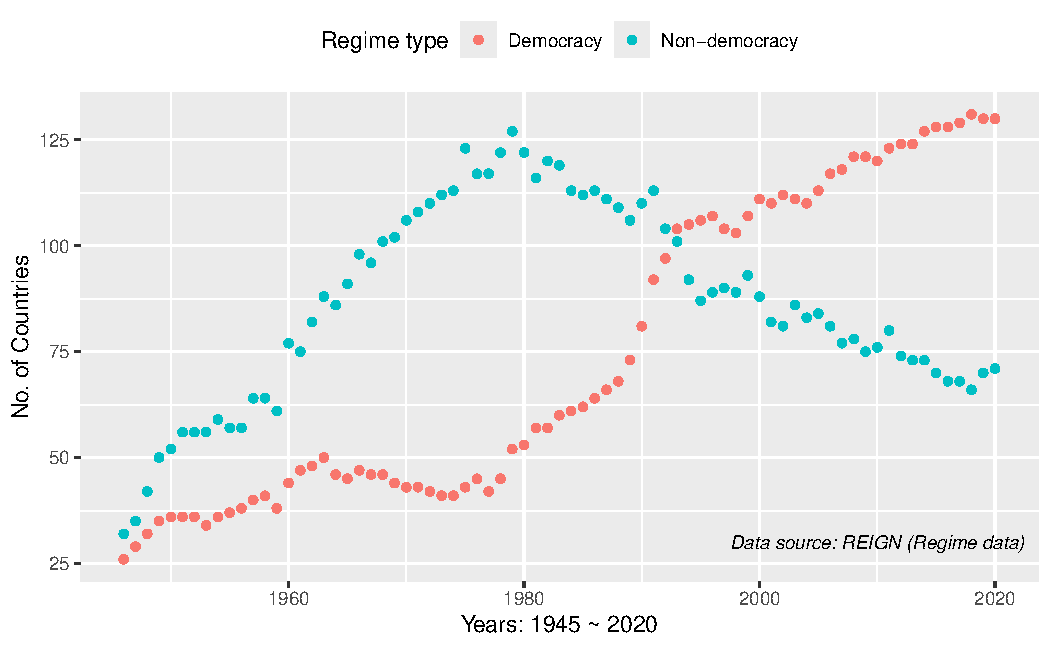
\includegraphics{coups_and_autocoups_files/figure-pdf/fig-democracy-1.pdf}

}

\caption{\label{fig-democracy}Comparison of the number of democratic and
non-democratic countries (1945-2020)}

\end{figure}%

However, a ``democratic recession'' has emerged in recent years
(\citeproc{ref-diamond2008}{Diamond 2008}). Freedom House reports an
18th consecutive year of global freedom decline in 2023
(\citeproc{ref-freedomhouse2024freedom}{Freedom House 2024}). While few
countries have completely regressed to autocracy, the average global
democracy level has fallen back to pre-2000 levels. Notably, democratic
backsliding often occurs within regimes, with democracies becoming less
liberal and autocracies becoming less competitive
(\citeproc{ref-mechkova2017}{Mechkova, Lührmann, and Lindberg 2017}).

This research highlights irregular power transitions as a significant
factor in democratic backsliding within regimes. These transitions,
often coups or autocoups, violate democratic norms and disrupt the path
towards stable democracies. Leaders who gain power through irregular
means often resort to undemocratic tactics to maintain control, creating
a vicious cycle of eroding democratic institutions.

Our findings suggest that the shorter lifespans and potentially severe
consequences associated with coups may deter potential coup leaders.
Conversely, autocoups appear to be a more tempting option for
power-hungry leaders due to their higher success rates, seemingly
moderate consequences, and extended leader tenure after the autocoup.
This trend may explain the decline in classic coups since the 1990s
alongside the rise of autocoups (\citeproc{ref-bermeo2016}{Bermeo
2016}).

\section{Limitations and directions for future
research}\label{limitations-and-directions-for-future-research}

This study offers a novel framework for analysing irregular power
transitions, but some limitations require further exploration:

\begin{itemize}
\item
  \textbf{Data refinement:} Defining and classifying autocoups is a new
  approach. Future research should validate this classification system
  through additional studies and expert evaluations.
\item
  \textbf{Data harmonization:} The current analysis faces challenges due
  to mismatched units (country-year vs.~leader) between coup and
  autocoup datasets. Future efforts should explore data harmonization
  techniques for more robust comparisons.
\item
  \textbf{Democratic backsliding:} While this study establishes a
  connection between irregular power transitions and democratic
  backsliding, further empirical evidence is needed to solidify this
  link.
\end{itemize}

Several avenues exist for future research:

\begin{itemize}
\item
  \textbf{Terminology and data collection:} Refining the ``autocoup''
  concept and achieving wider recognition will facilitate more accurate
  and comprehensive data collection.
\item
  \textbf{Dataset expansion:} Expanding the autocoup dataset with more
  cases and integrating it with data on other irregular leadership
  transitions can provide a more holistic view of political survival
  after these events.
\item
  \textbf{Power dynamics and long-term impacts:} Utilizing this dataset,
  future studies can delve deeper into power dynamics at play and
  explore the long-term consequences of irregular transitions on
  political systems, particularly regarding democratic backsliding,
  breakdown, and personalization of power.
\end{itemize}

In conclusion, this study sheds light on the dynamics of irregular power
transitions, specifically focusing on coups and autocoups. By redefining
autocoups, classifying the dataset, analysing determinants, and
comparing leader longevity, we establish a framework for understanding
irregular transitions and leader survival. This work contributes to a
deeper understanding of democratic resilience and political stability.
Future research can build upon this foundation by conducting further
empirical analyses based on the novel autocoup dataset and continuing to
refine the framework.

\newpage

\chapter*{References}\label{references}
\addcontentsline{toc}{chapter}{References}

\phantomsection\label{refs}
\begin{CSLReferences}{1}{0}
\bibitem[\citeproctext]{ref-aidt2019}
Aidt, Toke, and Gabriel Leon. 2019. {``The Coup.''} Edited by Roger D.
Congleton, Bernard Grofman, and Stefan Voigt, February.
\url{https://doi.org/10.1093/oxfordhb/9780190469771.013.15}.

\bibitem[\citeproctext]{ref-antonio2021}
Antonio, Robert J. 2021. {``Democracy and Capitalism in the Interregnum:
Trump{'}s Failed Self-Coup and After.''} \emph{Critical Sociology} 48
(6): 937--65. \url{https://doi.org/10.1177/08969205211049499}.

\bibitem[\citeproctext]{ref-marginaleffects}
Arel-Bundock, Vincent, Noah Greifer, and Andrew Heiss. NaN. {``How to
Interpret Statistical Models Using
{\textbraceleft}Marginaleffects{\textbraceright} in
{\textbraceleft}r{\textbraceright} and
{\textbraceleft}Python{\textbraceright},''} NaN.

\bibitem[\citeproctext]{ref-baturo2014}
Baturo, Alexander. 2014. {``Democracy, Dictatorship, and Term Limits.''}
\url{https://doi.org/10.3998/mpub.4772634}.

\bibitem[\citeproctext]{ref-baturo2019}
---------. 2019. {``Continuismo in Comparison.''} In, 75--100. Oxford
University Press.
\url{https://doi.org/10.1093/oso/9780198837404.003.0005}.

\bibitem[\citeproctext]{ref-baturo2022}
Baturo, Alexander, and Jakob Tolstrup. 2022. {``Incumbent Takeovers.''}
\emph{Journal of Peace Research} 60 (2): 373--86.
\url{https://doi.org/10.1177/00223433221075183}.

\bibitem[\citeproctext]{ref-bermeo2016}
Bermeo, Nancy. 2016. {``On Democratic Backsliding.''} \emph{Journal of
Democracy} 27 (1): 5--19. \url{https://doi.org/10.1353/jod.2016.0012}.

\bibitem[\citeproctext]{ref-bomprezzi2024wedded}
Bomprezzi, Pietro, Axel Dreher, Andreas Fuchs, Teresa Hailer, Andreas
Kammerlander, Lennart Kaplan, Silvia Marchesi, Tania Masi, Charlotte
Robert, and Kerstin Unfried. 2024. {``Wedded to Prosperity? Informal
Influence and Regional Favoritism.''} Discussion Paper. CEPR.

\bibitem[\citeproctext]{ref-brown2001}
Brown, Stephen. 2001. {``Authoritarian Leaders and Multiparty Elections
in Africa: How Foreign Donors Help to Keep Kenya's Daniel Arap Moi in
Power.''} \emph{Third World Quarterly} 22 (5): 725--39.
\url{https://doi.org/10.1080/01436590120084575}.

\bibitem[\citeproctext]{ref-cameron1998a}
Cameron, Maxwell A. 1998a. {``Latin American Autogolpes : Dangerous
Undertows in the Third Wave of Democratisation.''} \emph{Third World
Quarterly} 19 (2): 219--39.
\url{https://doi.org/10.1080/01436599814433}.

\bibitem[\citeproctext]{ref-cameron1998}
Cameron, Maxwell A. 1998b. {``Self-Coups: Peru, Guatemala, and
Russia.''} \emph{Journal of Democracy} 9 (1): 125--39.
\url{https://doi.org/10.1353/jod.1998.0003}.

\bibitem[\citeproctext]{ref-cassani2020}
Cassani, Andrea. 2020. {``Autocratisation by Term Limits Manipulation in
Sub-Saharan Africa.''} \emph{Africa Spectrum} 55 (3): 228--50.
\url{https://doi.org/10.1177/0002039720964218}.

\bibitem[\citeproctext]{ref-chaisty2019}
Chaisty, Paul. 2019. {``The Uses and Abuses of Presidential Term Limits
in Russian Politics.''} In, 385--402. Oxford University PressOxford.
\url{https://doi.org/10.1093/oso/9780198837404.003.0019}.

\bibitem[\citeproctext]{ref-cheeseman2015}
Cheeseman, Nic. 2015. {``Democracy in Africa,''} March.
\url{https://doi.org/10.1017/cbo9781139030892}.

\bibitem[\citeproctext]{ref-cheeseman2019}
---------. 2019. {``Should I Stay or Should I Go? Term Limits,
Elections, and Political Change in Kenya, Uganda, and Zambia.''} In,
311--38. Oxford University PressOxford.
\url{https://doi.org/10.1093/oso/9780198837404.003.0016}.

\bibitem[\citeproctext]{ref-cheeseman2019a}
Cheeseman, Nic, and Brian Klaas. 2019. \emph{How to Rig an Election}.
Yale University Press. \url{https://doi.org/10.12987/9780300235210}.

\bibitem[\citeproctext]{ref-chin2021}
Chin, John J, David B Carter, and Joseph G Wright. 2021. {``The
Varieties of Coups D{'}état: Introducing the Colpus Dataset.''}
\emph{International Studies Quarterly} 65 (4): 1040--51.
\url{https://doi.org/10.1093/isq/sqab058}.

\bibitem[\citeproctext]{ref-close2019}
Close, David. 2019. {``Presidential Term Limits in Nicaragua.''} In,
159--78. Oxford University PressOxford.
\url{https://doi.org/10.1093/oso/9780198837404.003.0009}.

\bibitem[\citeproctext]{ref-diamond2008}
Diamond, Larry. 2008. \emph{The Spirit of Democracy: The Struggle to
Build Free Societies Throughout the World}. Macmillan.

\bibitem[\citeproctext]{ref-ezrow2019}
Ezrow, Natasha. 2019. {``Term Limits and Succession in Dictatorships.''}
In, 269--88. Oxford University PressOxford.
\url{https://doi.org/10.1093/oso/9780198837404.003.0014}.

\bibitem[\citeproctext]{ref-fariss2022}
Fariss, Christopher J., Therese Anders, Jonathan N. Markowitz, and
Miriam Barnum. 2022. {``New Estimates of Over 500 Years of Historic GDP
and Population Data.''} \emph{Journal of Conflict Resolution} 66 (3):
553--91. \url{https://doi.org/10.1177/00220027211054432}.

\bibitem[\citeproctext]{ref-frantz2016}
Frantz, Erica, and Elizabeth A. Stein. 2016. {``Countering Coups:
Leadership Succession Rules in Dictatorships.''} \emph{Comparative
Political Studies} 50 (7): 935--62.
\url{https://doi.org/10.1177/0010414016655538}.

\bibitem[\citeproctext]{ref-freedomhouse2024freedom}
Freedom House. 2024. {``Freedom in the World 2024.''}
\url{https://freedomhouse.org/sites/default/files/2024-02/FIW_2024_DigitalBooklet.pdf}.

\bibitem[\citeproctext]{ref-gassebner2016}
Gassebner, Martin, Jerg Gutmann, and Stefan Voigt. 2016. {``When to
Expect a Coup d{'}état? An Extreme Bounds Analysis of Coup
Determinants.''} \emph{Public Choice} 169 (3-4): 293--313.
\url{https://doi.org/10.1007/s11127-016-0365-0}.

\bibitem[\citeproctext]{ref-geddes1999}
Geddes, Barbara. 1999. {``What Do We Know About Democratization After
Twenty Years?''} \emph{Annual Review of Political Science} 2 (1):
115--44. \url{https://doi.org/10.1146/annurev.polisci.2.1.115}.

\bibitem[\citeproctext]{ref-geddes2014}
Geddes, Barbara, Joseph Wright, and Erica Frantz. 2014. {``Autocratic
Breakdown and Regime Transitions: A New Data Set.''} \emph{Perspectives
on Politics} 12 (2): 313--31.
\url{https://doi.org/10.1017/s1537592714000851}.

\bibitem[\citeproctext]{ref-ginsburg2019}
Ginsburg, Tom, and Zachary Elkins. 2019. {``One Size Does Not Fit
All.''} In, 37--52. Oxford University Press.
\url{https://doi.org/10.1093/oso/9780198837404.003.0003}.

\bibitem[\citeproctext]{ref-ginsburg2010evasion}
Ginsburg, Tom, James Melton, and Zachary Elkins. 2010. {``On the Evasion
of Executive Term Limits.''} \emph{Wm. \& Mary L. Rev.} 52: 1807.

\bibitem[\citeproctext]{ref-ginsburg2011evasion}
---------. 2011. {``On the Evasion of Executive Term Limits.''}
\emph{William and Mary Law Review} 52: 1807.

\bibitem[\citeproctext]{ref-goemans2009}
Goemans, Henk E., Kristian Skrede Gleditsch, and Giacomo Chiozza. 2009.
{``Introducing Archigos: A Dataset of Political Leaders.''}
\emph{Journal of Peace Research} 46 (2): 269--83.
\url{https://doi.org/10.1177/0022343308100719}.

\bibitem[\citeproctext]{ref-helmke2017}
Helmke, Gretchen. 2017. {``Institutions on the Edge,''} January.
\url{https://doi.org/10.1017/9781139031738}.

\bibitem[\citeproctext]{ref-huntington1991democratization}
Huntington, Samuel P. 1991. {``The Third Wave: Democratization in the
Late Twentieth Century.''} \emph{Norman, OK: University of Oklahoma}.

\bibitem[\citeproctext]{ref-klesner2019}
Klesner, Joseph L. 2019. {``The Politics of Presidential Term Limits in
Mexico.''} In, 141--58. Oxford University Press.
\url{https://doi.org/10.1093/oso/9780198837404.003.0008}.

\bibitem[\citeproctext]{ref-krishnarajan2019}
Krishnarajan, Suthan. 2019. {``Economic Crisis, Natural Resources, and
Irregular Leader Removal in Autocracies.''} \emph{International Studies
Quarterly} 63 (3): 726--41. \url{https://doi.org/10.1093/isq/sqz006}.

\bibitem[\citeproctext]{ref-landau2019}
Landau, David, Yaniv Roznai, and Rosalind Dixon. 2019. {``Term Limits
and the Unconstitutional Constitutional Amendment Doctrine.''} In,
53--74. Oxford University PressOxford.
\url{https://doi.org/10.1093/oso/9780198837404.003.0004}.

\bibitem[\citeproctext]{ref-leon2013a}
Leon, Gabriel. 2013. {``Loyalty for Sale? Military Spending and Coups
d{'}etat.''} \emph{Public Choice} 159 (3-4): 363--83.
\url{https://doi.org/10.1007/s11127-013-0124-4}.

\bibitem[\citeproctext]{ref-llanos2019}
Llanos, Mariana. 2019. {``The Politics of Presidential Term Limits in
Argentina.''} In, 473--94. Oxford University Press.
\url{https://doi.org/10.1093/oso/9780198837404.003.0023}.

\bibitem[\citeproctext]{ref-marshall2005current}
Marshall, Monty G. 2005. {``Current Status of the World's Major Episodes
of Political Violence.''} \emph{Report to Political Instability Task
Force.(3 February)}.

\bibitem[\citeproctext]{ref-marsteintredet2019a}
Marsteintredet, Leiv. 2019. {``Presidential Term Limits in Latin
America: {\emph{C}}.1820{\textendash}1985.''} In, 103--22. Oxford
University PressOxford.
\url{https://doi.org/10.1093/oso/9780198837404.003.0006}.

\bibitem[\citeproctext]{ref-marsteintredet2019}
Marsteintredet, Leiv, and Andrés Malamud. 2019. {``Coup with Adjectives:
Conceptual Stretching or Innovation in Comparative Research?''}
\emph{Political Studies} 68 (4): 1014--35.
\url{https://doi.org/10.1177/0032321719888857}.

\bibitem[\citeproctext]{ref-mauceri1995}
Mauceri, Philip. 1995. {``State Reform, Coalitions, and The Neoliberal
{\emph{Autogolpe}} in Peru.''} \emph{Latin American Research Review} 30
(1): 7--37. \url{https://doi.org/10.1017/s0023879100017155}.

\bibitem[\citeproctext]{ref-mechkova2017}
Mechkova, Valeriya, Anna Lührmann, and Staffan I. Lindberg. 2017. {``How
Much Democratic Backsliding?''} \emph{Journal of Democracy} 28 (4):
162--69. \url{https://doi.org/10.1353/jod.2017.0075}.

\bibitem[\citeproctext]{ref-neto2019}
Neto, Octavio Amorim, and Igor P. Acácio. 2019. {``Presidential Term
Limits as a Credible-Commitment Mechanism.''} In, 123--40. Oxford
University PressOxford.
\url{https://doi.org/10.1093/oso/9780198837404.003.0007}.

\bibitem[\citeproctext]{ref-nurumov2019}
Nurumov, Dmitry, and Vasil Vashchanka. 2019. {``Presidential Terms in
Kazakhstan.''} In, 221--46. Oxford University PressOxford.
\url{https://doi.org/10.1093/oso/9780198837404.003.0012}.

\bibitem[\citeproctext]{ref-peyton2024}
Peyton, Buddy, Joseph Bajjalieh, Dan Shalmon, Michael Martin, and Emilio
Soto. 2024. {``Cline Center Coup d{'}état Project Dataset.''} University
of Illinois at Urbana-Champaign.
\url{https://doi.org/10.13012/B2IDB-9651987_V7}.

\bibitem[\citeproctext]{ref-pion-berlin2022}
Pion-Berlin, David, Thomas Bruneau, and Richard B. Goetze. 2022. {``The
Trump Self-Coup Attempt: Comparisons and Civil{\textendash}Military
Relations.''} \emph{Government and Opposition} 58 (4): 789--806.
\url{https://doi.org/10.1017/gov.2022.13}.

\bibitem[\citeproctext]{ref-posner}
Posner, Daniel N., and Daniel J. Young. n.d. {``Term Limits: Leadership,
Political Competition and the Transfer of Power.''} In, 260--78.
Cambridge University Press.
\url{https://doi.org/10.1017/9781316562888.011}.

\bibitem[\citeproctext]{ref-powell2012}
Powell, Jonathan. 2012. {``Determinants of the Attempting and Outcome of
Coups d{'}état.''} \emph{Journal of Conflict Resolution} 56 (6):
1017--40. \url{https://doi.org/10.1177/0022002712445732}.

\bibitem[\citeproctext]{ref-powell2011}
Powell, Jonathan M, and Clayton L Thyne. 2011. {``Global Instances of
Coups from 1950 to 2010: A New Dataset.''} \emph{Journal of Peace
Research} 48 (2): 249--59.
\url{https://doi.org/10.1177/0022343310397436}.

\bibitem[\citeproctext]{ref-powell2018}
Powell, Jonathan, Christopher Faulkner, William Dean, and Kyle Romano.
2018. {``Give Them Toys? Military Allocations and Regime Stability in
Transitional Democracies.''} \emph{Democratization} 25 (7): 1153--72.
\url{https://doi.org/10.1080/13510347.2018.1450389}.

\bibitem[\citeproctext]{ref-przeworski2000}
Przeworski, Adam, Michael E. Alvarez, Jose Antonio Cheibub, and Fernando
Limongi. 2000. {``Democracy and Development,''} August.
\url{https://doi.org/10.1017/cbo9780511804946}.

\bibitem[\citeproctext]{ref-reyntjens2016}
Reyntjens, Filip. 2016. {``A New Look at the Evidence.''} \emph{Journal
of Democracy} 27 (3): 61--68.
\url{https://doi.org/10.1353/jod.2016.0044}.

\bibitem[\citeproctext]{ref-roessler2011}
Roessler, Philip. 2011. {``The Enemy Within: Personal Rule, Coups, and
Civil War in Africa.''} \emph{World Politics} 63 (2): 300--346.
\url{https://doi.org/10.1017/s0043887111000049}.

\bibitem[\citeproctext]{ref-singh2016}
Singh, Naunihal. 2016. \emph{Seizing Power}. Johns Hopkins University
Press. \url{https://doi.org/10.1353/book.31450}.

\bibitem[\citeproctext]{ref-stinnett2002}
Stinnett, Douglas M., Jaroslav Tir, Paul F. Diehl, Philip Schafer, and
Charles Gochman. 2002. {``The Correlates of War (Cow) Project Direct
Contiguity Data, Version 3.0.''} \emph{Conflict Management and Peace
Science} 19 (2): 59--67.
\url{https://doi.org/10.1177/073889420201900203}.

\bibitem[\citeproctext]{ref-sudduth2017}
Sudduth, Jun Koga. 2017. {``Strategic Logic of Elite Purges in
Dictatorships.''} \emph{Comparative Political Studies} 50 (13):
1768--1801. \url{https://doi.org/10.1177/0010414016688004}.

\bibitem[\citeproctext]{ref-svolik2014}
Svolik, Milan W. 2014. {``Which Democracies Will Last? Coups, Incumbent
Takeovers, and the Dynamic of Democratic Consolidation.''} \emph{British
Journal of Political Science} 45 (4): 715--38.
\url{https://doi.org/10.1017/s0007123413000550}.

\bibitem[\citeproctext]{ref-tangri2010}
Tangri, Roger, and Andrew M. Mwenda. 2010. {``President Museveni and the
Politics of Presidential Tenure in Uganda.''} \emph{Journal of
Contemporary African Studies} 28 (1): 31--49.
\url{https://doi.org/10.1080/02589000903542574}.

\bibitem[\citeproctext]{ref-thyne2019}
Thyne, Clayton L., and Jonathan Powell. 2019. {``Coup Research,''}
October. \url{https://doi.org/10.1093/acrefore/9780190846626.013.369}.

\bibitem[\citeproctext]{ref-sampleSelection-2}
Toomet, Ott, and Arne Henningsen. 2008. {``Sample Selection Models in
{\textbraceleft}r{\textbraceright}: Package
{\textbraceleft}sampleSelection{\textbraceright}''} 27.
\url{https://www.jstatsoft.org/v27/i07/}.

\bibitem[\citeproctext]{ref-versteeg2020law}
Versteeg, Mila, Timothy Horley, Anne Meng, Mauricio Guim, and Marilyn
Guirguis. 2020. {``The Law and Politics of Presidential Term Limit
Evasion.''} \emph{Colum. L. Rev.} 120: 173.

\end{CSLReferences}



\end{document}
